\chapter{Experimental Results and Evaluations}
\label{chap:k3}

\cref{sec:Materials} provides information about the used dataset. 

\cref{sec:ParameterSelection} describes the chosen parameters for line extraction, line projection on DSM, and window sliding processes.

In \cref{sec:simulation}, the correctness of the derived LS model for reconstruction is evaluated. Some other properties of the proposed reconstruction approach are also discussed.

\cref{sec:truedata} evaluates the true data results. The result of single continuous lane-marking is presented and the theoretical precision is evaluated.
%The distance between the LIDAR points and the generated DSM are computed and evaluated statistically
%To evaluate the influence of the over-counting correction and MGM
%cost aggregation independently, two evaluations were performed

\clearpage
%%%%%%%%%%%%%%%%%%%%%%%%%%%%%%%%%%%%%%%%%%%%%%%%%%%%%%%%
\section{Materials}
\label{sec:Materials}

\paragraph{Aerial Images}
For real-time mapping applications during disasters, mass events and traffic monitoring scenarios, the German Aerospace Center (DLR) has developed a new optical sensor system-- the 4k system-- operated on a helicopter from DLR. The oblique aerial images used in this work are acquired from a Canon EOS 1D-X camera, one of the three non-metric cameras in the 4k system, with an oblique viewing angle $\tau$ of 15$\degree$. The pixel size is around $6.9$ \textmu m, with the combination of focal length $50$ mm and flying height $H_{flight}$ around $500$ m above ground, leading to a GSD of $\sim$6.9 cm.

As described in \cite{Fischer2017}, this aerial imagery shall be improved to have an absolute geolocation accuracy of better than 30 centimeters if TerraSAR-X geodetic points are included as reference points.

An example aerial image is shown in \cref{fig:OriImg}. \cref{tab:CameraProperties} lists the properties of this camera, and \cref{tab:SensorViewingGeometry} provides the viewing geometry information.
\begin{figure}
	\centering
	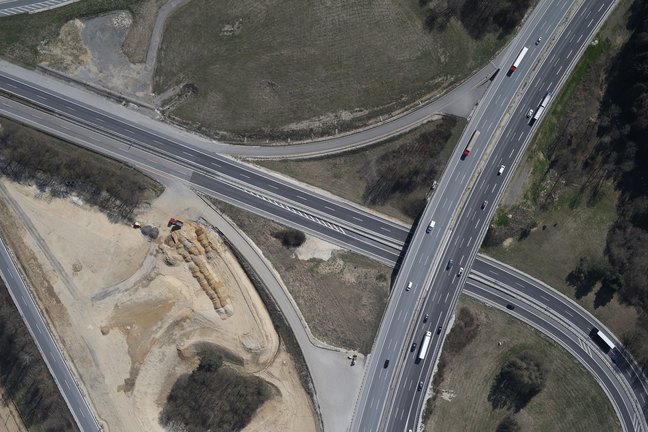
\includegraphics[width=0.8\textwidth]{L1234_rsz.png}
	\caption{\small Original Image}
	\label{fig:OriImg}
\end{figure}

\begin{table}%[!h]
  \centering
  \begin{tabular}{ll}
  \toprule
                                      {} & \textbf{Canon EOS 1D-X} \\
  \midrule
  Lenses                          & Zeiss Makro Planar f/2.0\;50mm\\
  \\[-1em]
  Sensor / Pixel size             & Full frame CMOS / 6.944 \textmu m\\
  \\[-1em]
  \multirow{2}{*}{Image size}     & 5184$\times$3456 pixel, ratio 3:2\\
                                  & (17.9 MPix)\\
  \\[-1em]
  ISO                             & 100--204800\\
  \\[-1em]
  max. frame rate / max. images   & 14 fps/ 180 images\\
  \\[-1em]
  Exposure time                   & 30 s -- 1/8000 s\\
  \\[-1em]
  Data interface                  & LAN (EDSDK software interface)\\
  \bottomrule
  \end{tabular}
  \caption{Properties of the oblique camera }
  \label{tab:CameraProperties}
\vspace{0.5cm}
  \centering
  \begin{tabular}{lll}
  \toprule
                         & \textbf{RGB, 50mm lens} \\
  \midrule
  Oblique angle          & $\pm$15$\degree$\\
  \\[-1em]
  \multirow{2}{*}{FOV}   & $\pm$34$\degree$ across strip,\\
                         & $\pm$13$\degree$ along strip\\
  \\[-1em]
  Coverage @500m         & 780 m $\times$ 230 m\\
  GSD      @500m         & 6.9 cm (nadir)\\

  \bottomrule
  \end{tabular}
  \caption{Viewing geometry}
  \label{tab:SensorViewingGeometry}
\end{table}

The images used in this work are acquired with a special flight configuration at both sides of the motorway which guarantees a continuous stereo view perpendicular to the lane marking direction.\footnote{The classical photogrammetric approach on flight planning is to have several straight flight lines which cover the whole motorway in a stereo view. This would be possible in this project yet would require more flight costs and would produce many more images.} This is realized by flying at the right-hand side with respect to flying direction along the motorway, with the left oblique camera looking left-down to the motorway, in both forward and backward trips. The flight configuration is shown in \cref{fig:FlightTrajectory} on the Google Earth platform.

\begin{figure}%[!h]
	\centering
	\subfloat[]{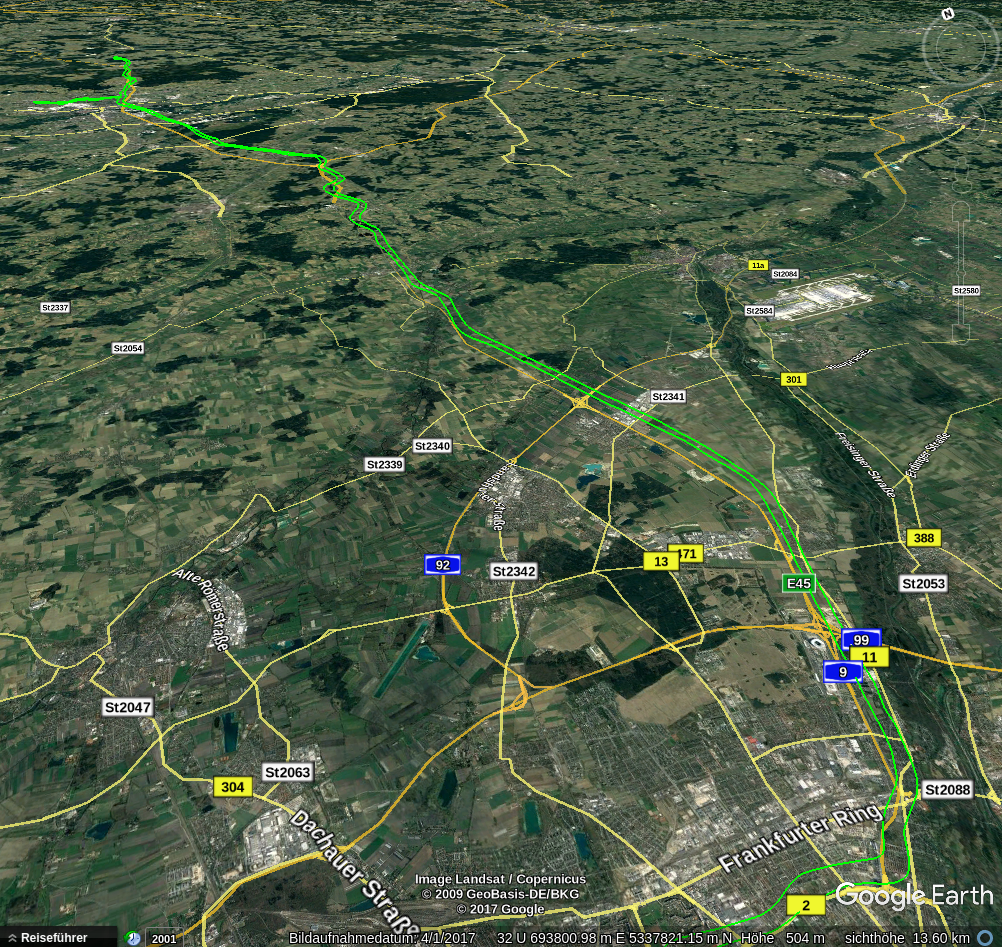
\includegraphics[height=0.5\textwidth]{FlightTrajectory5.png} \label{fig:trajectory1}}
	\subfloat[]{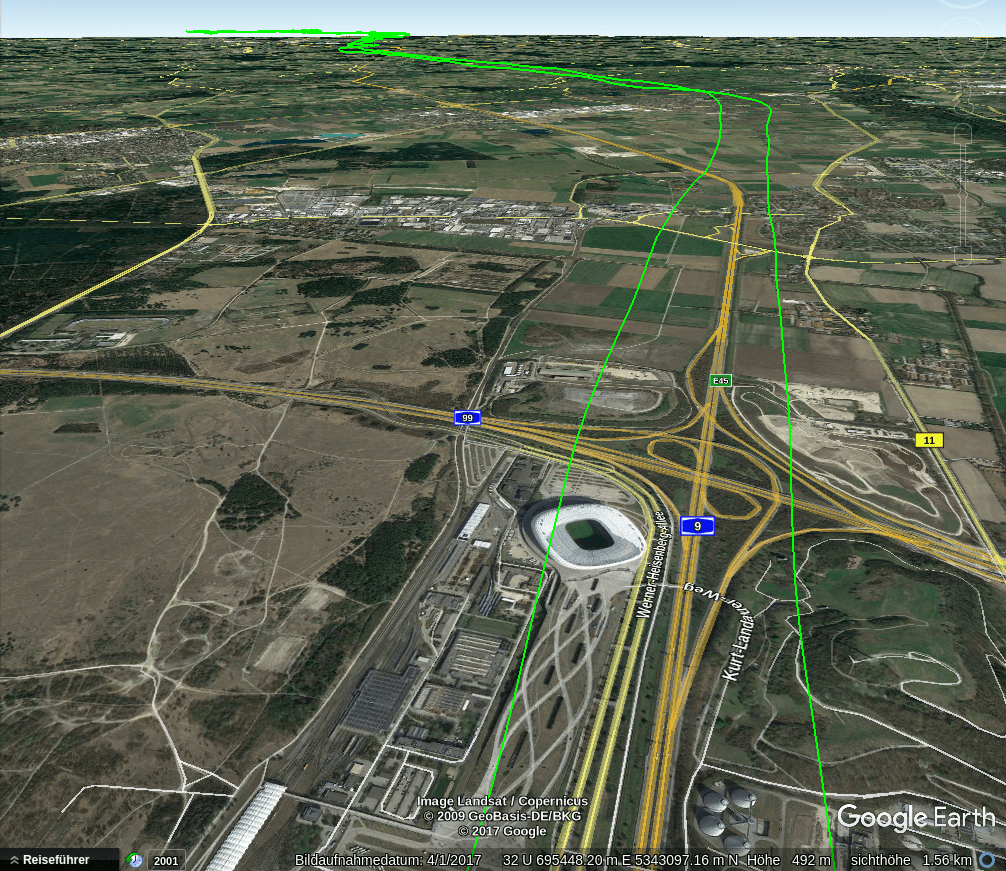
\includegraphics[height=0.5\textwidth, trim=220 0 0 0,clip]{FlightTrajectory3.png} \label{fig:trajectory2}}
	\caption{\small Flight trajectory of DLR helicopter visualized on the Google Earth platform. The green polyline shows the flight trajectory. \textit{Source: \textbf{Google Earth} 04/01/2017}}
	\label{fig:FlightTrajectory}
\end{figure}

\clearpage
There are 15 images used in this work: 8 images in forward trip (first strip) and 7 in backward (second strip). The length of flight strips is around 590 meter.

Besides, the forward overlap is around 70\%, and all the lane markings are covered by both strips, whereas the side overlap depends on the distance of flight strips, which is a result of the pilots navigation ability and other influences, like wind. Nevertheless, the motorway in its entire width was covered by the two flight strips. Altogether, this results in approximately 8-image coverage in road areas. 


\paragraph{Exterior and Interior Orientations}
The aerial images are geo-referenced by \gls{gnss}/Inertial system IGI AEROcontrol-IId and further improved by \gls{sapos} correction. Additionally, a global terrain modell (from SRTM mission) was introduced as pass information in the bundle adjustment, to improve the estimation of the focal length and boresight alignment. Self-calibrating bundle adjustment is applied to calibrate \gls{io} parameters and to refine \gls{eo} parameters. \cref{tab:EOprecision} and \cref{tab:IOprecision} show the precision of IO and EO parameters after self-calibrating bundle adjustment. % Missing: specification of the system, ,….
To provide an overall quality on the interior orientations: from the calibration result of interior orientations (involving lens distortion), the residuals appear non-systematic and the biggest residual $r_{max, IO}$ is around 1 pixel.% 1 pixel可彙整入表3.4,改正數無系統性如果要寫出來,需繪圖證明。

\begin{table}[!h]
	\centering
	\begin{tabular}{ll|ll}
		\toprule
		position precisions  &[meter]  & attitude precisions & [degree]\\
		\midrule
		$\sigma_{north}$     & $0.055$ & $\sigma_{roll}$  & $0.002$\\
		$\sigma_{east}$      & $0.035$ & $\sigma_{pitch}$ & $0.002$\\
		$\sigma_{altitude}$  & $0.069$ & $\sigma_{yaw}$   & $0.005$\\
		\bottomrule
	\end{tabular}
	\caption{Precisions of Exterior Orientations}
	\label{tab:EOprecision}
	\vspace{0.5cm}
	\centering
	\begin{tabular}{lr|lr|l}
		\toprule
		\multicolumn{2}{c|}{Interior Orientations}  & \multicolumn{2}{c|}{precisions} & unit\\
		\midrule
		focal length $c$                       &   $0.051$ & $\sigma_c$      & $6.9\mathrm{e}{-7}$ & [meter]\\
		x coordinate of principal point $pp_x$ & $-42.259$ & $\sigma_{pp_x}$ & $0.167$             &[$\mu$m]\\
		x coordinate of principal point $pp_y$ & $115.384$ & $\sigma_{pp_y}$ & $0.799$             &[$\mu$m]\\
		\bottomrule
	\end{tabular}
	\caption{Interior Orientations and their precisions}
	\label{tab:IOprecision}
\end{table}


\clearpage
To evaluate the influence of the uncertainties in exterior and interior parameters on positioning precision in object space, the maximum values for each component based on the flight configuration was calculated.
The quality of interior and exterior orientation parameters set would have a maximum impact in object space for around $16$ [cm] in X,Y-direction:
\begin{itemize}
      \item caused by inaccurate camera position: 
      \item [] $\sqrt{\sigma_{north}^2+\sigma_{east}^2}=\sqrt{0.055^2+0.035^2}\approx0.065$ [meter]
      \item caused by inaccurate camera attitude, as illustrated in :
      \item [] $ H_{flight}\times\sqrt{(\tan(\sigma_{roll}+\tau)-\tan\tau)^2+(\dfrac{\tan\sigma_{pitch}}{\cos\tau})^2}$
      \item [] $=500\times\sqrt{(\tan(0.002\degree+15\degree)-\tan15\degree)^2+(\dfrac{\tan0.002\degree}{\cos15\degree})^2}\approx0.026$ [meter]
      \item caused by inaccurate Interior Orientations:
      \item [] $r_{max, IO}\times GSD=1\times0.069=0.069$ [meter]
\end{itemize}
and around $6.9$ [cm] in Z-direction:
\begin{itemize}
      \item caused by inaccurate camera position:
      \item [] $\sigma_{altitude}\approx0.069$ [meter]
%      \item caused by inaccurate camera attitude:
%      \item [] $H_{flight}\times\dfrac{\tan(\sigma_{roll}+\tau)-\tan\tau}{\tan(\sigma_{roll}+\tau)}$
%      \item [] $=500\times\dfrac{\tan(0.002\degree+15\degree)-\tan15\degree}{\tan(0.002\degree+15\degree)}\approx0.070$ [meter]
%      \item caused by inaccurate Interior Orientations:
%      \item [] $r_{max, IO}\times GSD\times\dfrac{\sin\tau}{\cos\tau}=1\times0.069\times\dfrac{\sin15\degree}{\cos15\degree}\approx0.018$ [meter]
\end{itemize}

\begin{figure}%[!h]
	\centering
	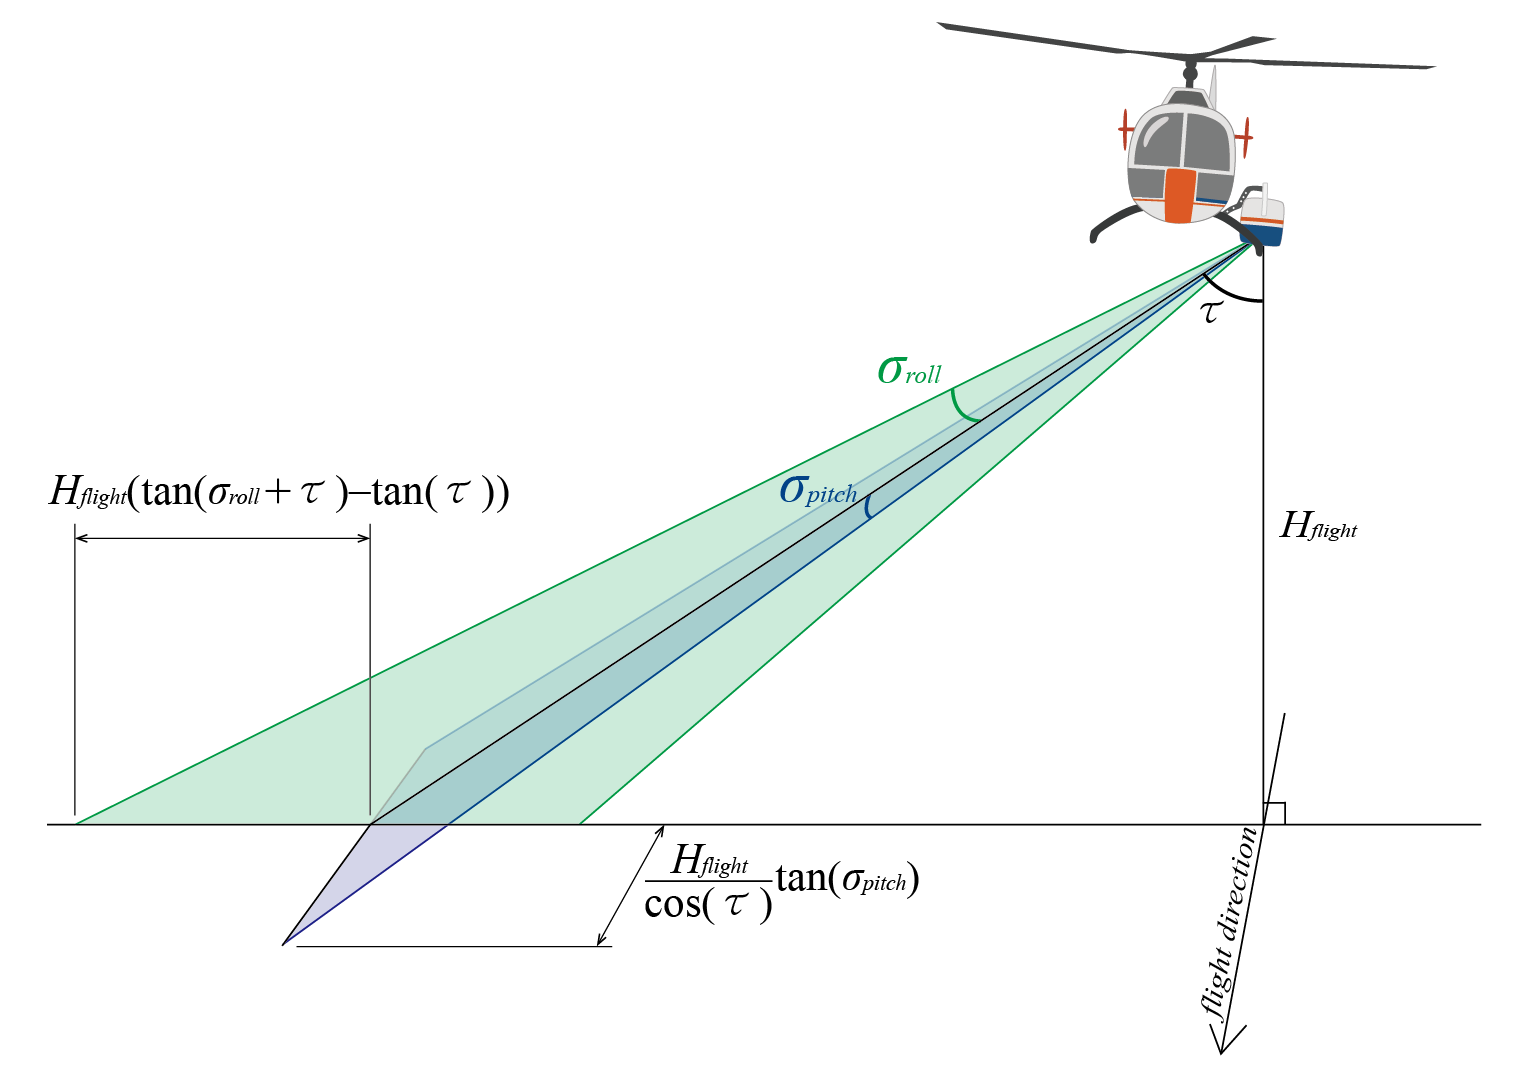
\includegraphics[width=0.9\textwidth]{EOinfluence-1.png}
	\caption{\small The impact of uncertain camera attitude in horizontal direction.}
	\label{fig:EOinfluence-1}
\end{figure}

The above information tells the positioning precision in object space with measurements on a single image. With corresponding measurements from MVS, which allows the intersection of multiple projection rays from different directions, the positioning precision is expected to be improved.% for being overdetermined.



\paragraph{\gls{dsm}}
The DSM used in this experiment is generated by SGM based on MVS. As the asphalt road surfaces on which the lane markings are located are poorly textured, the SGM generated DSM is especially noisy in such poorly textured areas. However, such high-resolution DSM gives a good starting point for the lane marking refinement. In other words, the DSM will be used only for setting up the initial values of the work flow, and will not influence the final results of the 3D lane marking reconstruction.

The DSM has 20 cm grid spacing. \cref{fig:DSM} shows a part of the DSM. Standard deviations of the height value in this part of the DSM is shown in \cref{fig:DSMstd}. The number of stereo image pairs used for each part on the DSM is shown in \cref{fig:DSMnumber}.

% Standard deviation not well visible. Maybe add number of images for this small part
% scale bar
\begin{figure}%[!h]
  \centering
  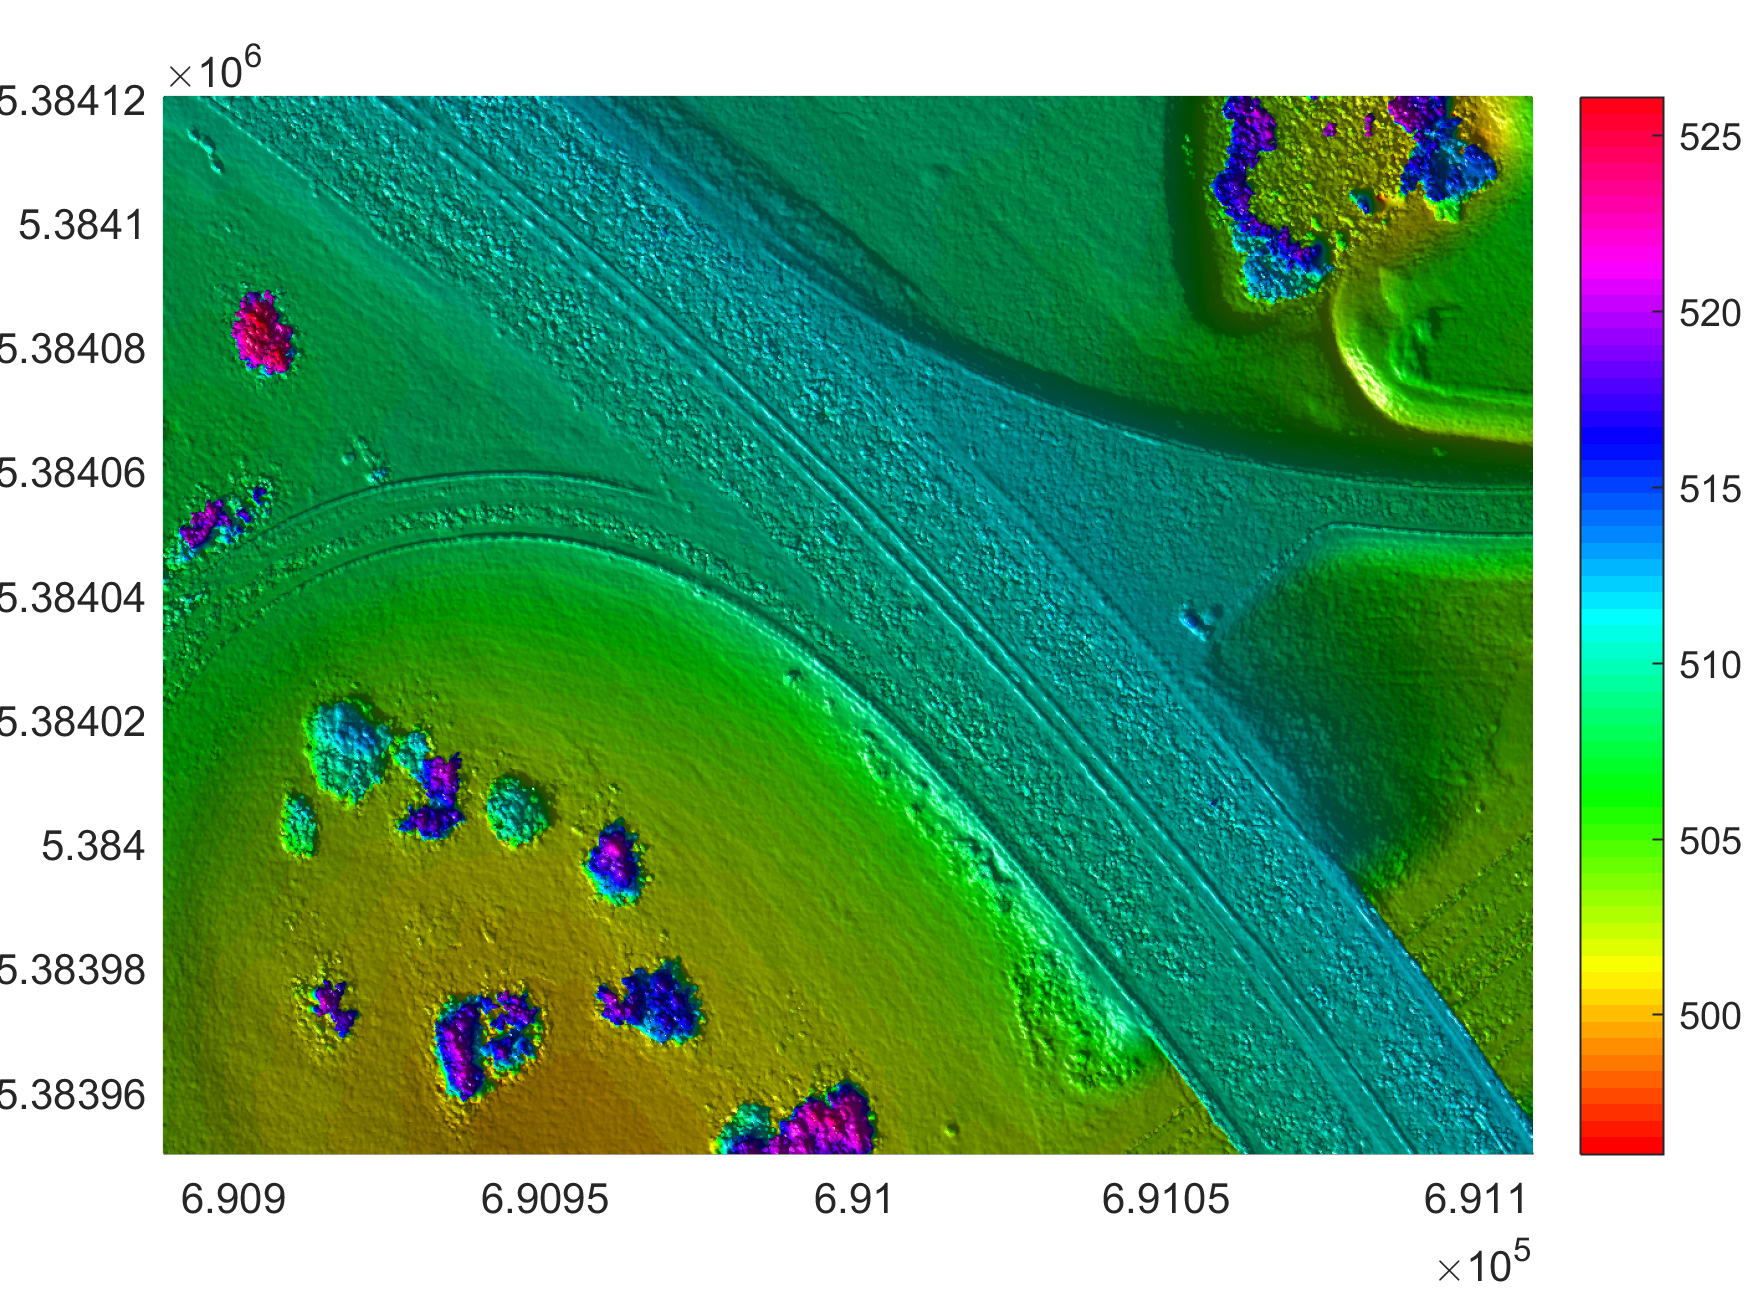
\includegraphics[width=0.9\textwidth]{DEM_A9_small_hsv.png}
  \caption{\small Part of the DSM in road area. It is noisy in the center of motorway.}
  \label{fig:DSM}
  \vspace{0.5cm}
  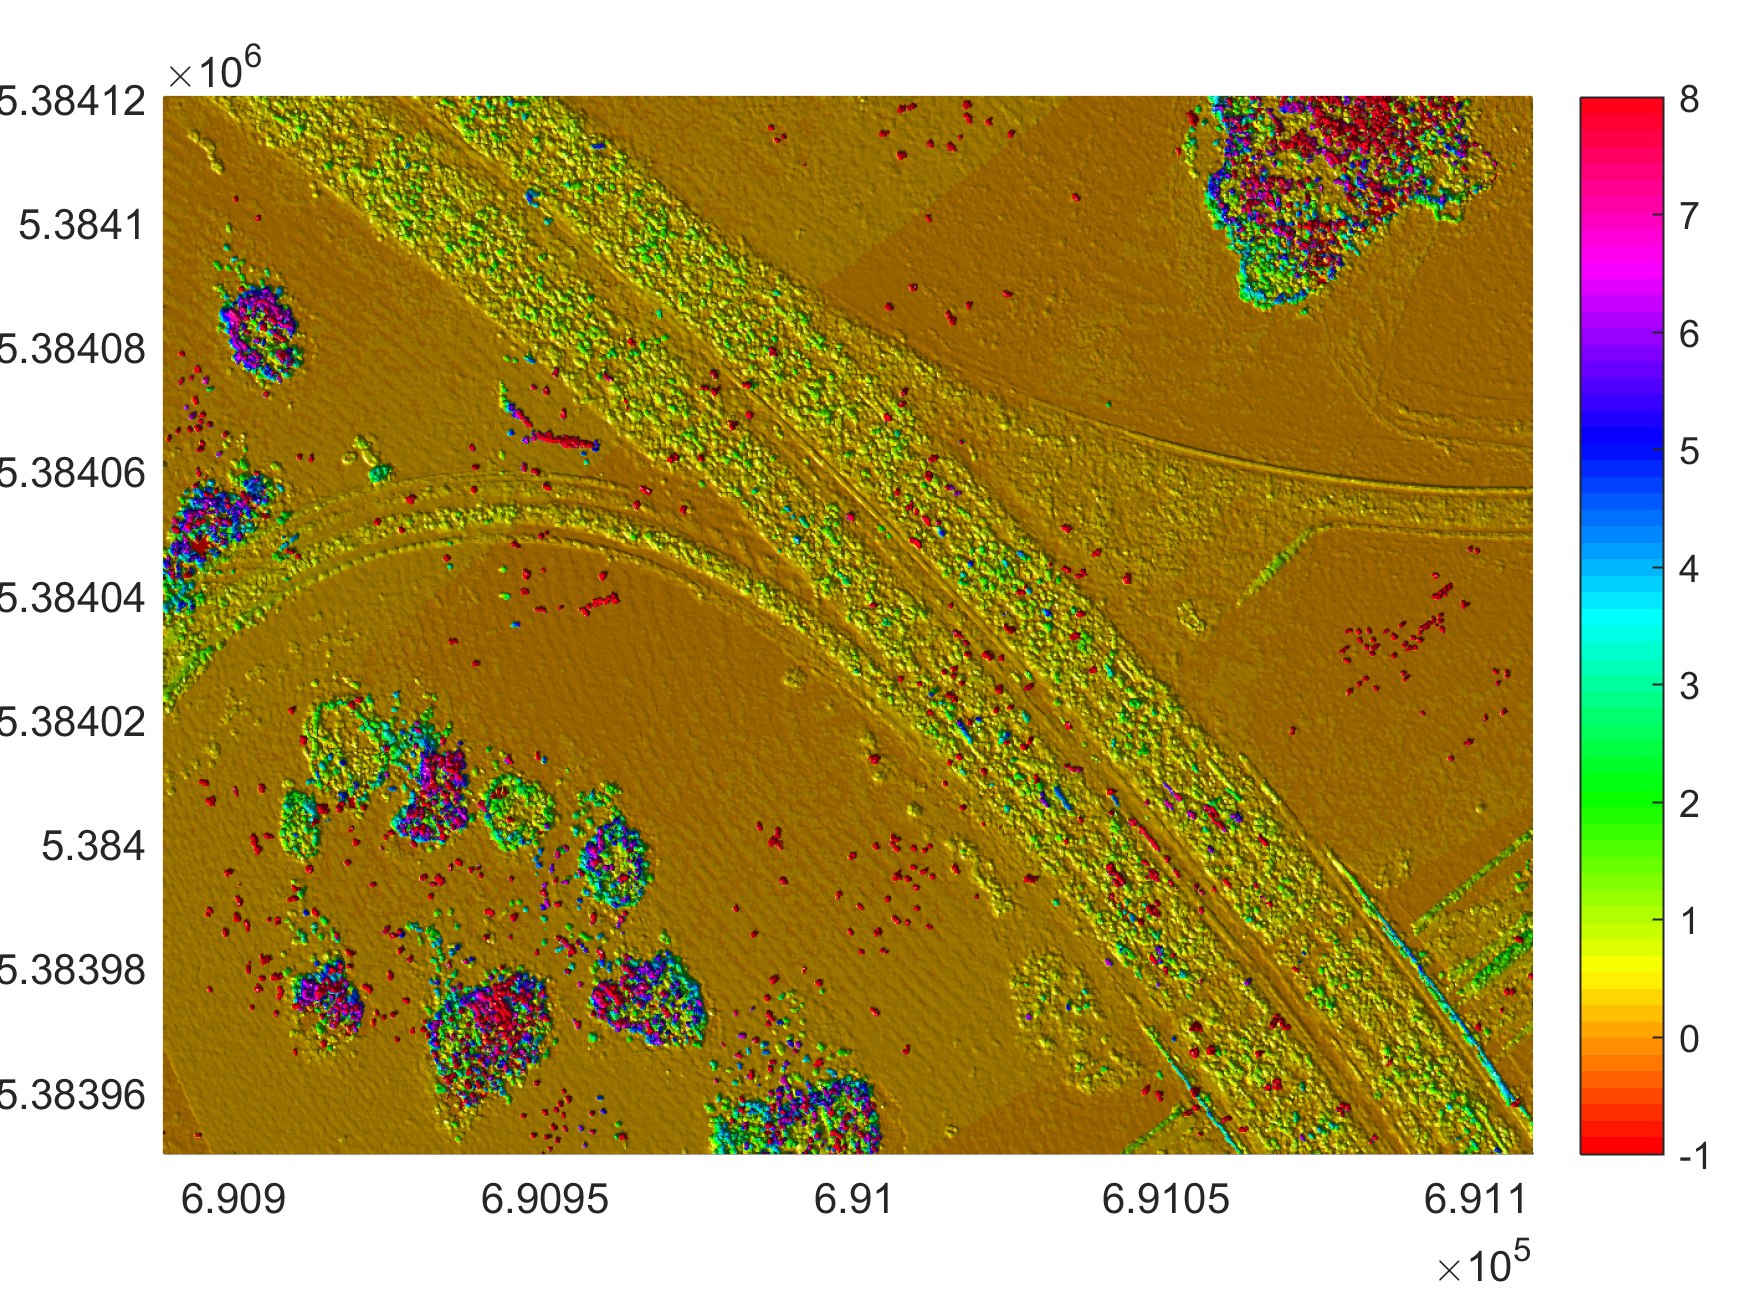
\includegraphics[width=0.9\textwidth]{DEM_A9_STD_small_hsv8.png}
  \caption{\small Standard deviations of the height value of the DSM in road area. It has higher value in the center of motorway.}
  \label{fig:DSMstd}

\end{figure}

\begin{figure}%[!h]
  \centering
  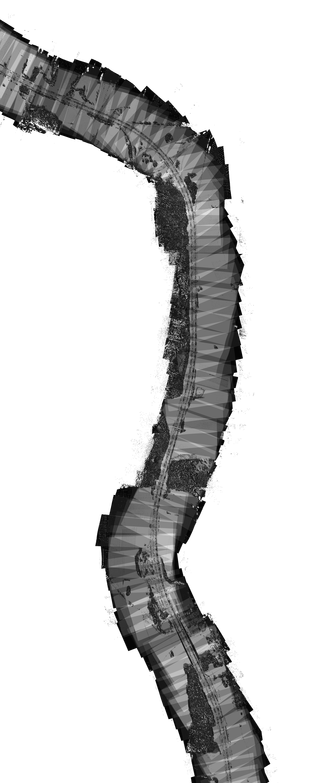
\includegraphics[width=0.5\textwidth]{DEM_A9_NUM_scaled_s.png}
  \caption{\small Distribution of stereo pairs used for DSM generation. Lighter color indicates more stereo pairs are used in that area. Maximum 27 stereo pairs are used for one pixel.}%%%%%%%%
  \label{fig:DSMnumber}
\end{figure}


\paragraph{Orthorectified Images}
The orthorectified images are processed using the DSM and the interior and exterior orientations derived from the bundle adjustment. One of the orthorectified images is shown in \cref{fig:OrthoImg}. The orthorectified images are only used for setting up initial values and used as intermediary step for processing the road masks, but do not influence the results of 3D lane marking reconstruction.
% Maybe a nice place, to visualize the DSM error on the lane marking projections…

\paragraph{Road Masks}
Road segments are masked out from original images based on \gls{osm} data: Firstly, the rasterized road segments from OSM data are written with 25 meter buffer width around road axes into orthorectified images. By back-projecting the mask from orthorectified image to original image using the 3D information from the DSM, it can then be used to mask out the road regions on the original images, as shown in \cref{fig:MaskedImg}.

\begin{figure}%[!h]
	\centering
    	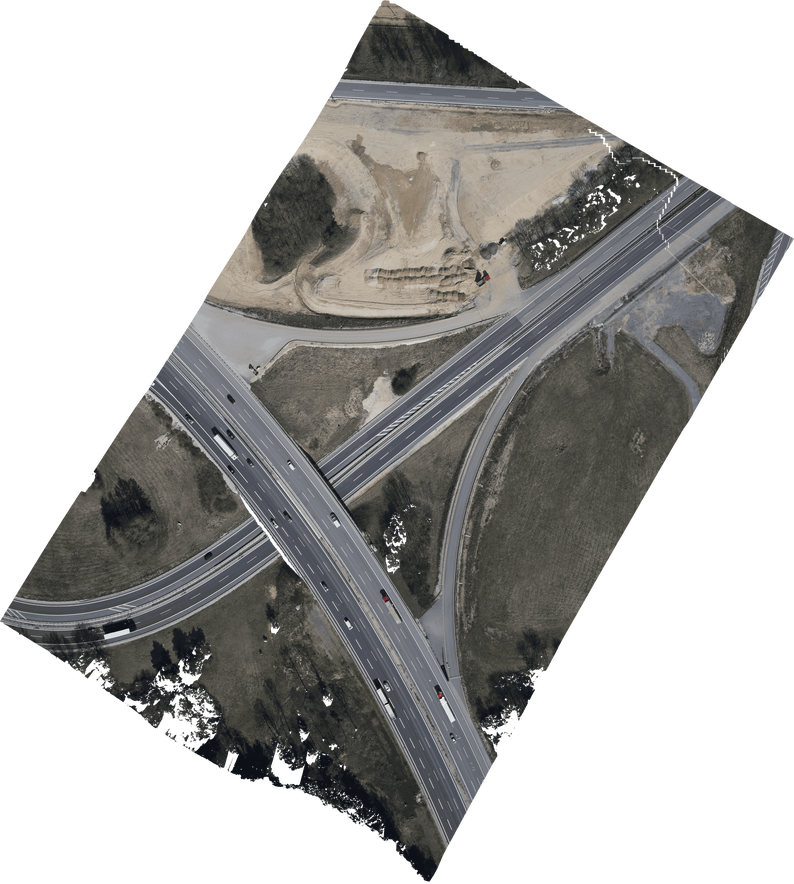
\includegraphics[width=0.8\textwidth]{OL1234_rsz.png}
    	\caption{\small Orthorectified Image}
    	\label{fig:OrthoImg}
	\vspace{0.5cm}
		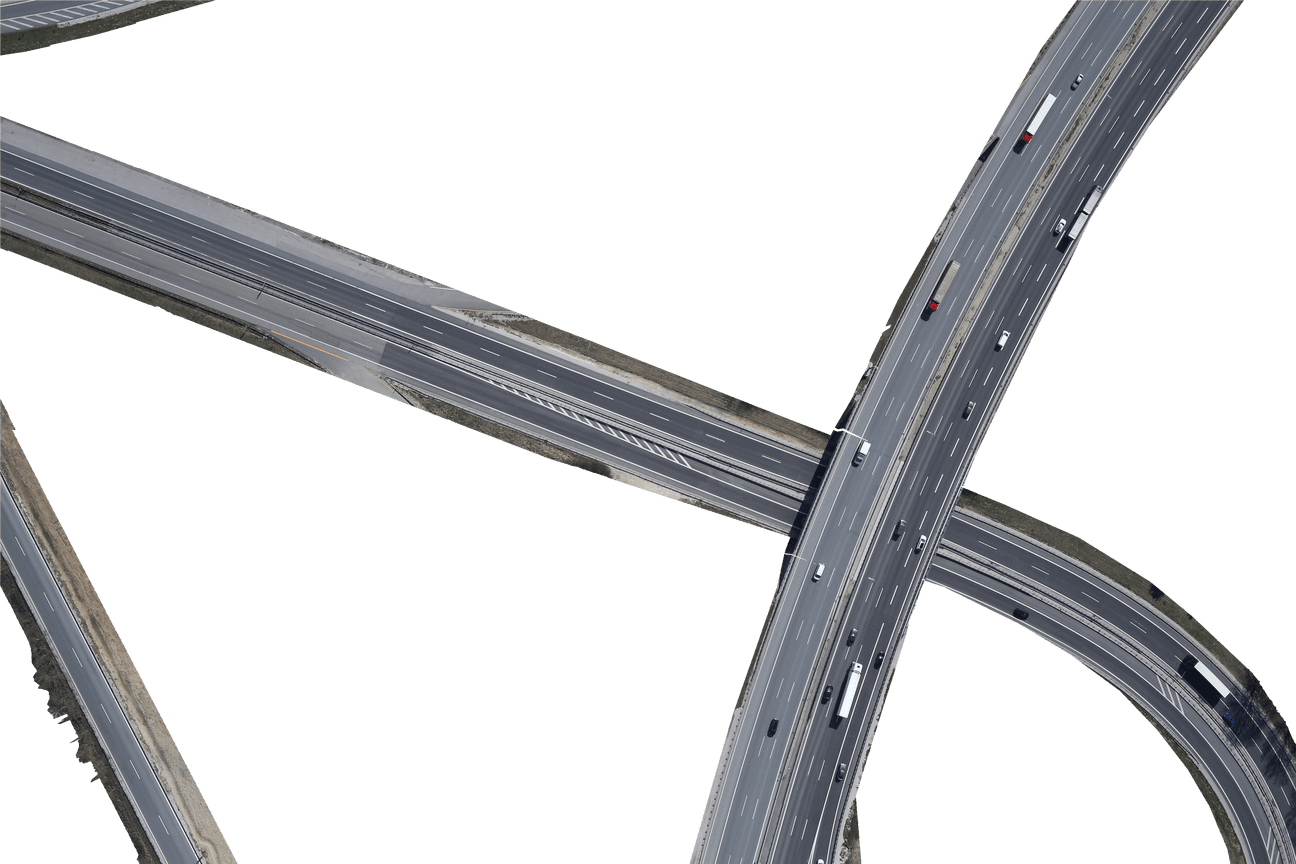
\includegraphics[width=0.75\textwidth]{ML1234_rsz.png}
		\caption{\small Masked Image}
		\label{fig:MaskedImg}
\end{figure}

\clearpage
%%%%%%%%%%%%%%%%%%%%%%%%%%%%%%%%%%%%%%%%%%%%%%%%%%%%%%%%
\section{Parameter Selection}
\label{sec:ParameterSelection}

%%% extraction %%%%%%%%%%%%%%%%
In lane marking extraction process (see \cref{sec:LineExtraction}), the $\sigma$ value for Gaussian smoothing is set to be 1.8 to slightly suppress the noise in images. % From HALCON Referenz: For the choice of the thresholds High and Low one has to keep in mind that the second directional derivative depends on the amplitude and width of the line as well as the choice of Sigma. Thus: you must set this value depending on the lane marking width?
A length threshold on the extracted lines is applied to reduce false positives ---the detected line features which are indeed not lane markings. Regarding the fact that a dashed lane-line is around 6 meter long which corresponds to 62--87 pixels in image space (when parallel to one of the coordinate axes or in 45$\degree$ direction), the extracted lines whose length is less than 65 pixels are rejected.
% http://www.mvtec.com/doc/halcon/11/en/lines_gauss.html
% https://www.dvr.de/download/publikationen-schriftenreihe-17.pdf


%%% line projection on DSM %%%%%%%%%%%%%%%%
The convergence threshold for 2D image point projection on DSM (see \cref{sec:LineProjectionOnDSM}) is selected as 0.5 m, as the height precision on road surface of the used DSM is expected to be around 50 cm.


%%% sliding window %%%%%%%%%%%%%%%%
The length of the sliding window should be decided base on the expected curvature of the targeted line and the robustness of the reconstruction model. In the cases of continuous lane markings on motorways, the sliding window length was fixed to 16 m, or for the last line segment it may be up to 24 m long, as a compromise between optimization robustness and the minimized systematic errors arisen from straight-approximated curvature. As to the cases of dashed lane-lines (6 m long), a sliding window has the same length as its targeted approximating line, i.e. it has 6 m length. The step size of sliding window was set to half of the sliding window length, i.e. 8 m.



%%% measurements collection: buffer width %%%%%%%%%%%%%%%%
%The 10 pixels buffering width corresponds to 70 cm in object space. the imperfect DSM profile has maximum ...which is around 70 cm in image space. 


%%% LS parameters %%%%%%%%%%%%%%%%
%convergence threshold 


%%% amount of image coverage %%%%%%%%%%%%%%%%


%%% lens distortion -> not straight line preserved
The adapted lens distortion model is none shape-preserving, i.e. a 3D straight line is no more straight in image. However in every independent reconstruction process, only a short 16 m line segment is reconstructed, whose lens distortion correction along this line segment is no bigger than one pixel. Thus the bending of a line segment on an image, arose from lens distortion, is ignored in this work, but could be easily removed from the images by rectifiying the images (i.e. calculating non distorted images).


%%%%%%%%%%%%%%%%%%%%%%%%%%%%%%%%%%%%%%%%%%%%%%%%%%%%%%%%
\section{Simulation}
\label{sec:simulation}
This section aims to verify the correctness of the derived LS model and to discover some characteristics of the reconstruction model using simulated data. The used materials are as described in \cref{sec:Materials}. Only the measurements (the image coordinates of the extracted lines) as well as the true and approximate values of the unknowns (the object coordinates of a line segment) in the non-linear LS model are simulated, as described in \cref{subsec:simudata}.

\cref{subsec:simuresult} firstly evaluates whether the iteration scheme converges to the correct solution given imperfect initial values of the unknowns. The significant height differences between the approximate and the reconstructed line segments are also presented, indicating the refining ability of the proposed reconstruction approach.

The ability of the derived LS model on detecting the measurement errors is then evaluated. Furthermore, the increase of covering images would influence on the reconstruction result is elaborated.

%Note that the quality of camera parameters (EO., IO. and additional parameters) do not have influences in simulation since the simulated measurements are produced with the same set of camera parameters as the set used for 3D reconstruction.




\subsection{Simulation Data}
\label{subsec:simudata}

\paragraph{The true line segment in object space}
Firstly, the object coordinates of the endpoints of a 3D line segment are defined, with 151.8 meters length, locating on the road surface in the test area (German highway A9) with 3 to 7 aerial images coverage. By linear interpolating several points with 0.2 meter spaces (considering DSM grid of 0.2 meter) between the two endpoints, a 3D line segment in the form of a set of 3D points is generated. This 3D line segment serves as the ground truth in the experiments in \cref{sec:simulation}. 

\paragraph{The observed line segments in image spaces}
The observations in the LS model are simulated by back-projecting the true line segment into the covering images. Gaussian random noise $e\sim\mathcal{N}(0,0.5^2)$ is added in the observations for each LS adjustment, as line extraction process is of sub-pixel accuracy. The added noise is plotted in \cref{fig:noise}

\begin{figure}
  \centering
  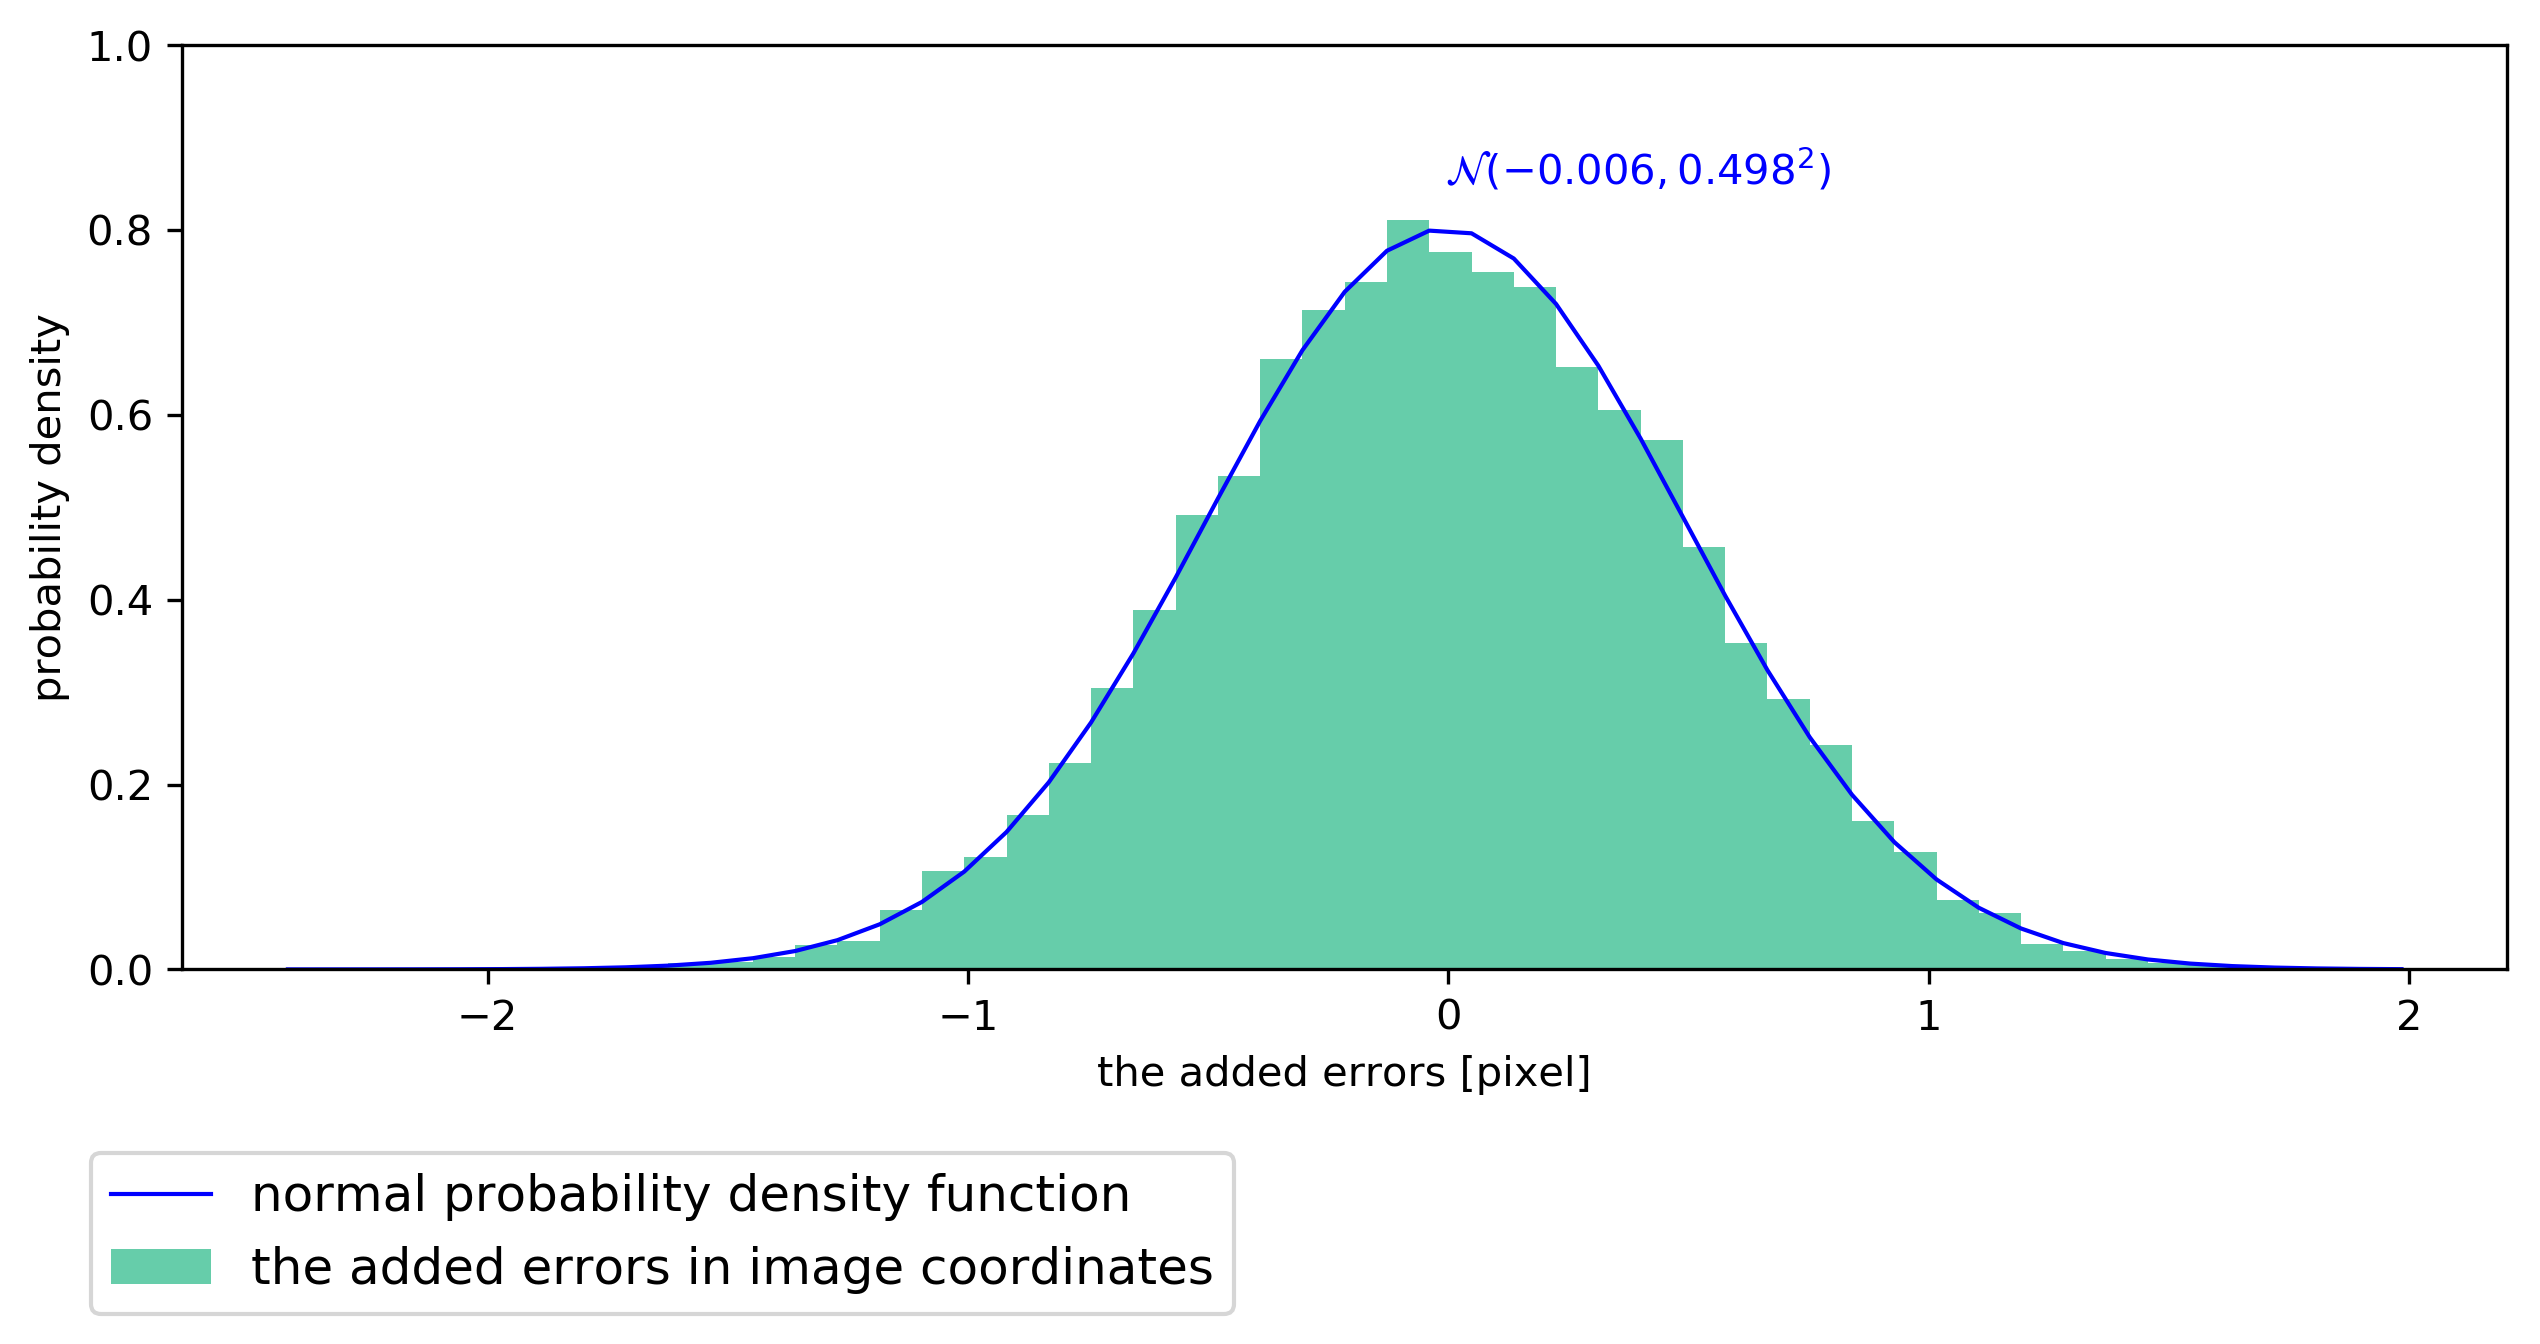
\includegraphics[width=\textwidth]{Simu_errorhist_1.png}
  \caption{\small The added Gaussian random noise in the observations.}
  \label{fig:noise}
\end{figure}

\paragraph{The approximate line segment in object space}
The initial estimates for non-linear LS adjustment is generated by projecting the observed line segments in image space onto the DSM.

\clearpage

\subsection{Simulation Result}
\label{subsec:simuresult}

%%% analysis on the unknowns:
\cref{fig:Simu3D_2} shows the reconstructed and the true line segments in UTM 32N coordinate system. The distances from the reconstructed line nodes to the true line segment are computed and collected, resulting in sample size of $18$. The sample mean is $0.008$ [meter] and the sample variance is $0.101^2$ [meter\textsuperscript{2}]. % This sampling procedure is assumed to be independent and random.%??? (t test assumptions)

For such small sample size data, a two-tailed t-test is adopted to test if the population mean significantly not equals zero, i.e. {if the reconstructed line segments are significantly far from the true line segments}. Null hypothesis ($H_0$) and (two-tailed) alternative hypothesis ($H_A$) are stated as:
\begin{equation*}
\begin{split}
H_0: \mu=0\\
H_A: \mu\neq0
\end{split}
\end{equation*}

A significance level $\alpha=0.05$ is selected, with degree of freedom being $18-1=17$, the two-tailed t-table value $T_{(0.975,17)}$ is
\begin{equation*}
T_{(0.975,17)}=2.110
\end{equation*}
which leads to the decision rule: if test statistic $T_{obs}$ is less than $-T_{(0.975,17)}=-2.110$ or greater than $T_{(0.975,17)}=2.110$, reject the null hypothesis.

With the sample mean $\overline{x}=0.008$ [meter],
the proposed population mean $\mu_0=0$ [meter],
the sample standard deviation $\sigma=0.101$ [meter],
and sample size $n=18$, the test statistic for One Sample T Test has the calculated value:
\begin{equation*}
T_{obs} = \frac{\overline{x}-\mu_0}{\sigma/\sqrt{n}}=\frac{0.008-0}{0.101/\sqrt{18}}\approx0.34
\end{equation*}
which is neither less than $-T_{(0.975,17)}=-2.110$ nor greater than $T_{(0.975,8)}=2.110$, i.e. not in the rejection region. As a result, we fail to reject the null hypothesis. In other words, {we are not able to claim that the reconstructed line is significantly far away from the true line}. This indicates that {the derived non-linear LS adjustment model for 3D reconstruction is correct}.

\cref{fig:Simu3D_1} shows the reconstructed line segments and the DSM profile which serves as the initial approximation for non-linear LS adjustment, in UTM 32N coordinate system. The maximum distance between them is 1.97 meter, mainly in Z-direction. This tells that {the reconstruction model is at least able to refine the initial approximation with 2 meters bias in Z-direction}.

\begin{figure}
  \centering
  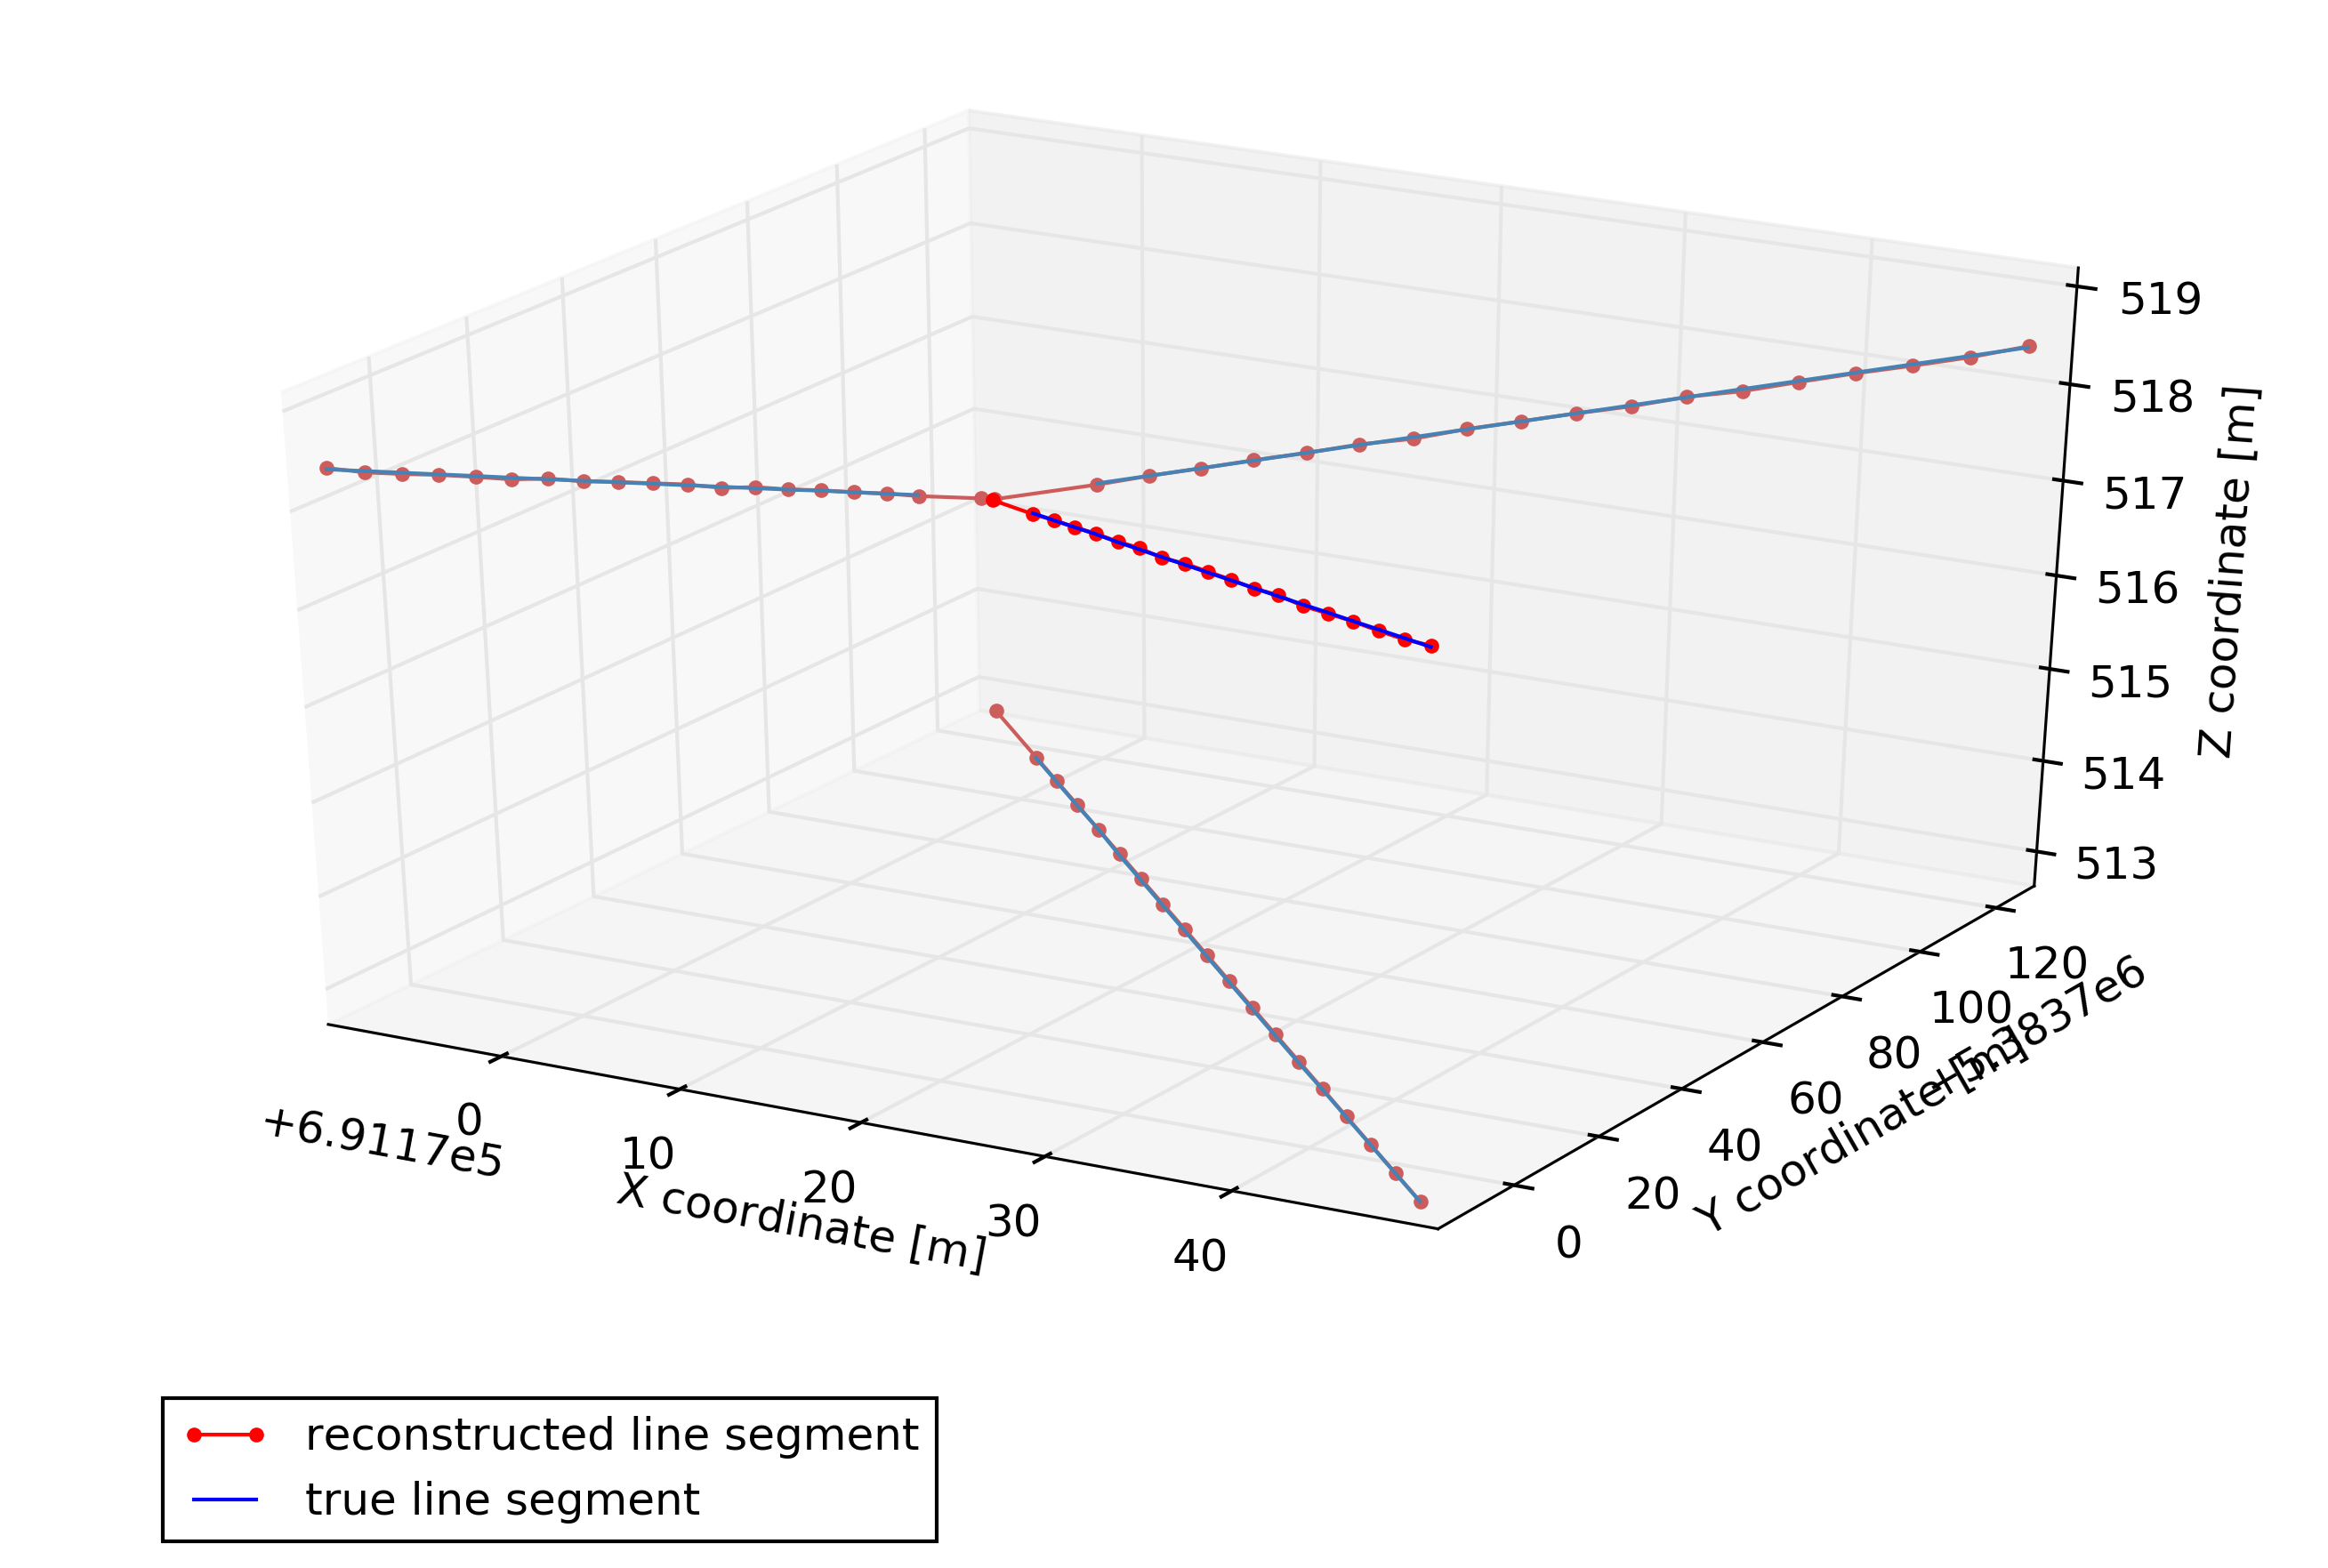
\includegraphics[width=\textwidth]{Simu_3D_2.png} %%% 換,字重疊。
  \caption{\small The reconstructed line segments and the true line segments in UTM 32N coordinate system.}
  \label{fig:Simu3D_2}
  \vspace{1cm}
  \centering
  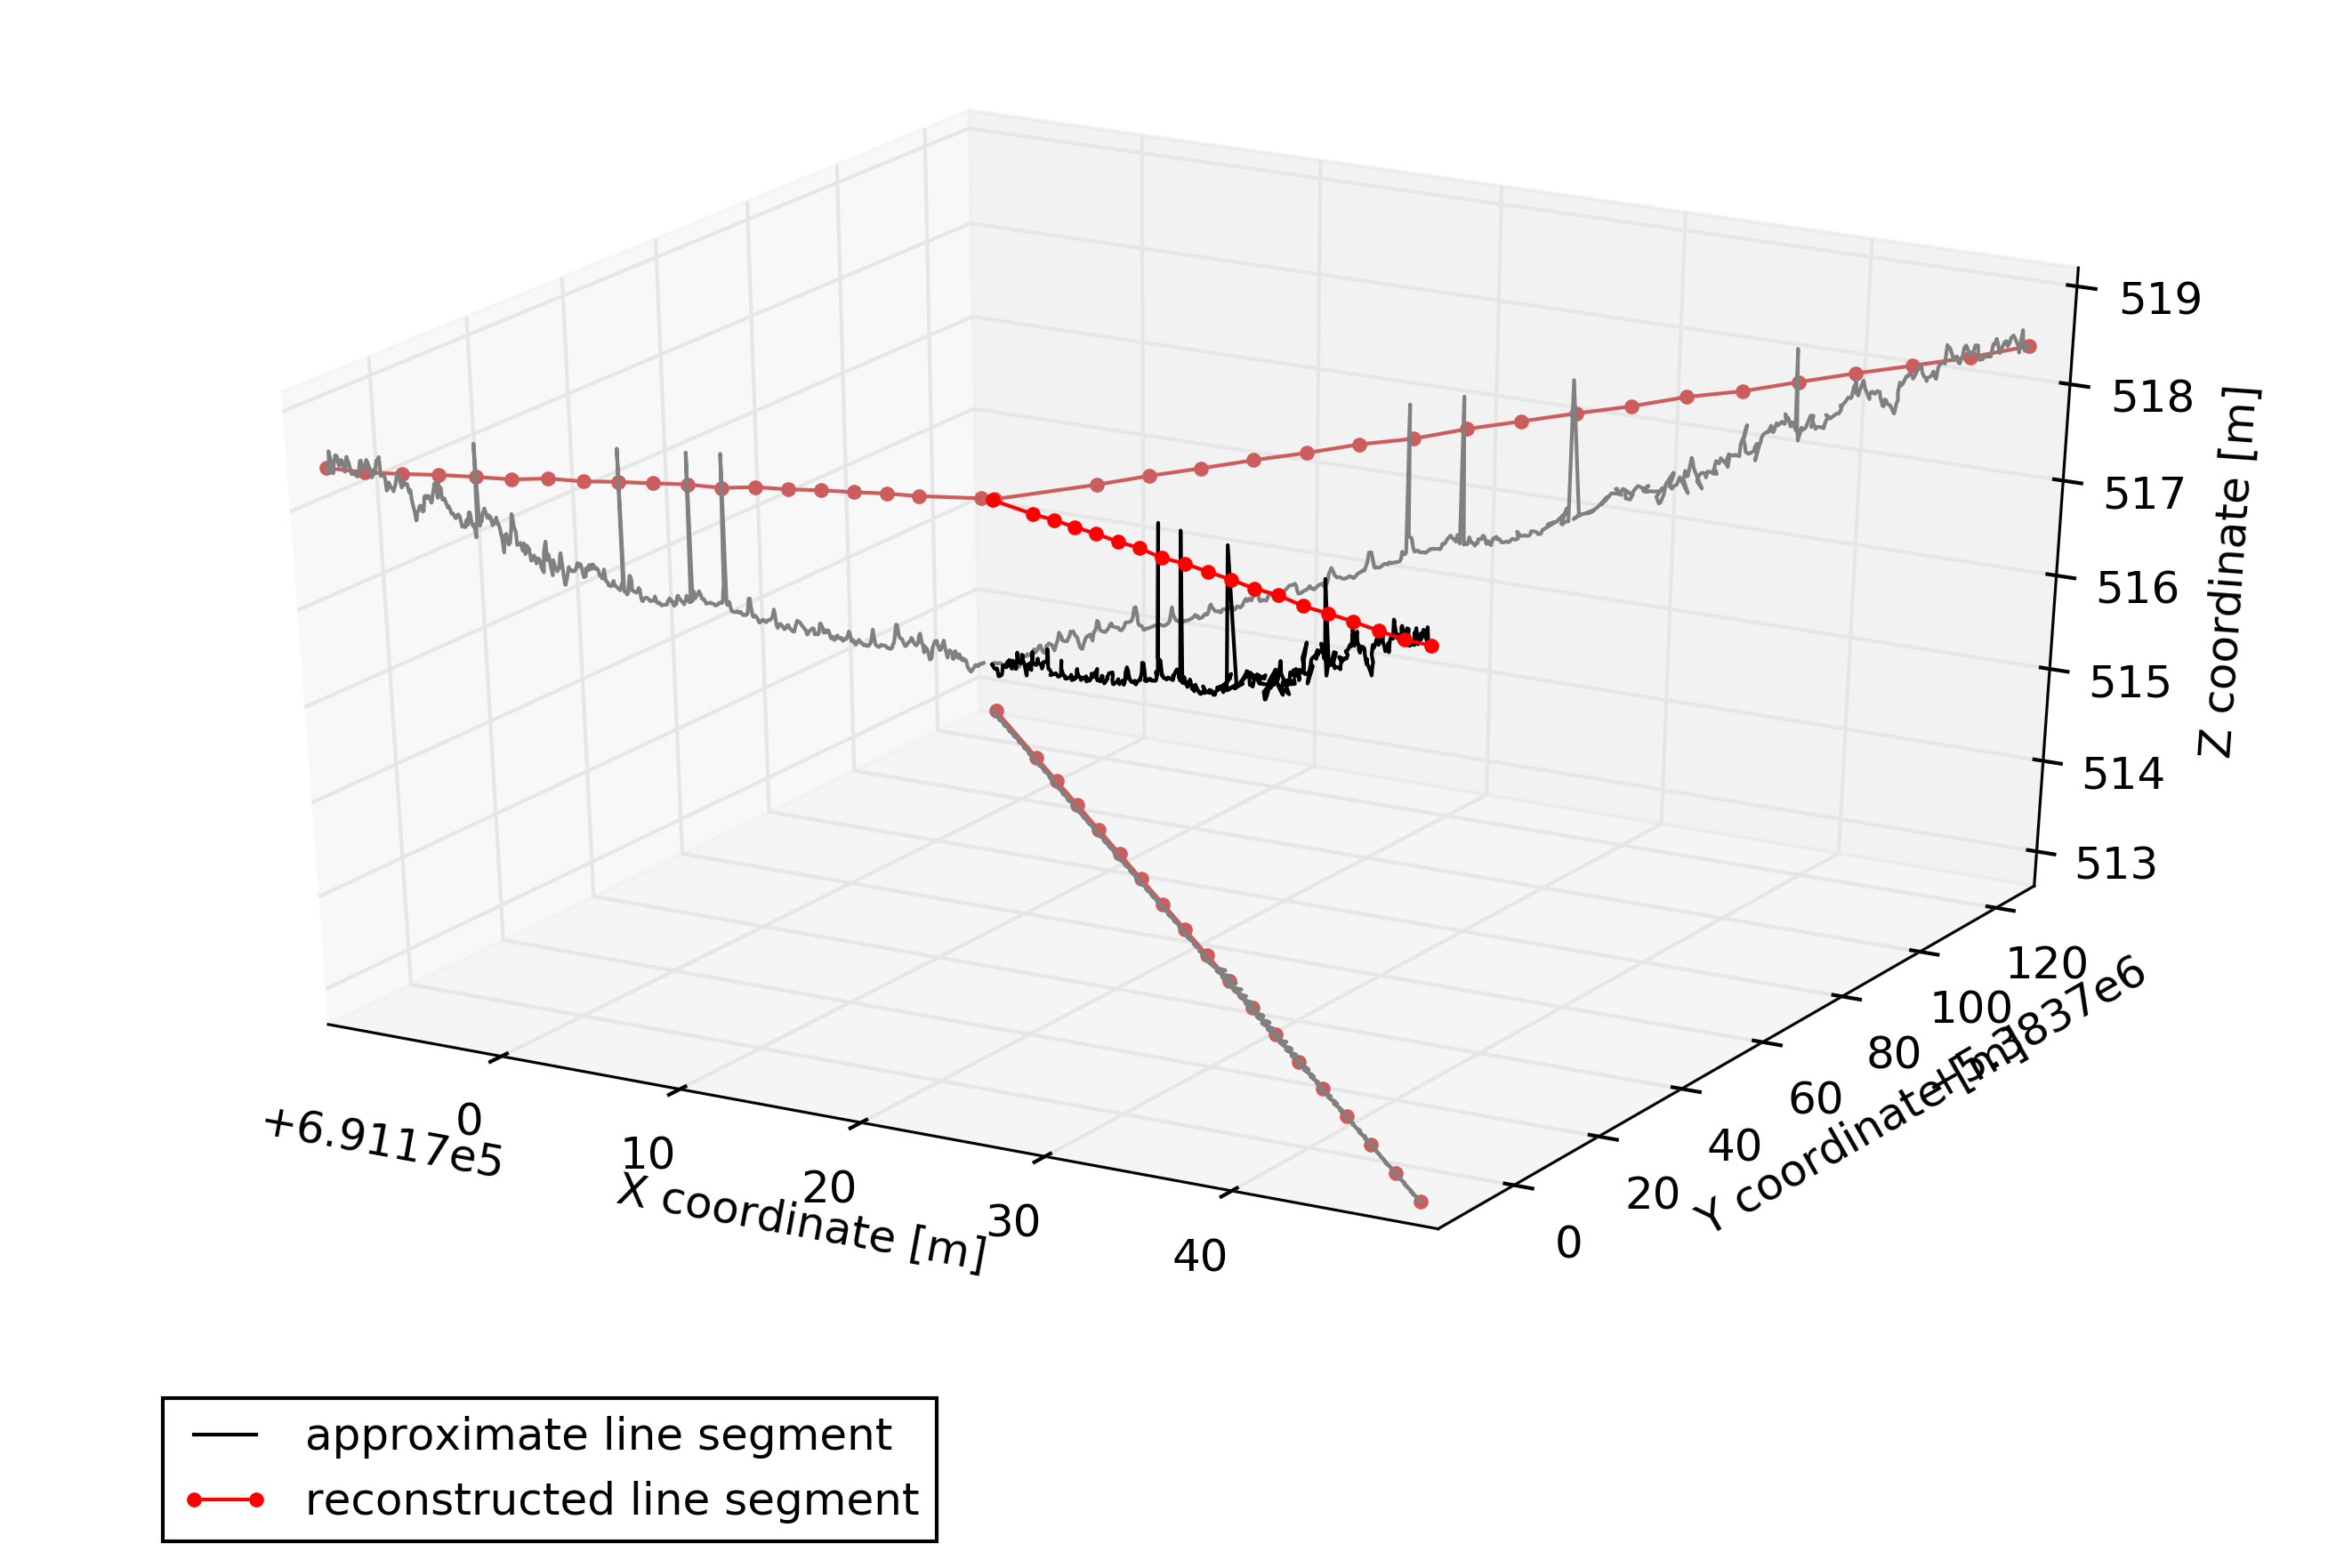
\includegraphics[width=\textwidth]{Simu_3D_1.png}
  \caption{\small The reconstructed line segments and the unrefined DSM profile in UTM 32N coordinate system.}
  \label{fig:Simu3D_1}
\end{figure}

\clearpage




%The distances from the reconstructed line segment to the DSM profile are plotted into histogram in \cref{fig:SimuHist_1}. They are collected along the reconstructed line segments with 0.2 meter spacing (considering the DSM grid of 0.2 meter), resulting in sample size of $381$. The sample mean is $-0.029$ [meter] and the sample variance is $0.083$ [meter]. % This sampling procedure is assumed to be independent and random.%??? and normal distributed (Z test assumptions)

%In order to know \textbf{if the mean distance from the reconstructed line segments to the DSM profile is significantly non-zero}, a two-tailed Z-test is adopted for such big sample size cases. Null hypothesis ($H_0$) and (two-tailed) alternative hypothesis ($H_A$) are stated as:
%\begin{equation*}
%\begin{split}
%H_0: \mu=0\\
%H_A: \mu\neq0
%\end{split}
%\end{equation*}

%A significance level $\alpha=0.05$ is selected, which is $0.025$ on each tail of the population, i.e. the area in body is $0.975$ out of 100\%. The corresponding z-score is:
%\begin{equation*}
%Z_{0.975}=1.96
%\end{equation*}
%which leads to the decision rule: if $Z_{obs}$ is less than $-1.96$ or greater than $1.96$, reject the null hypothesis.

%With the sample mean $\overline{x}=-0.029$,
%the proposed population mean $\mu_0=0$,
%the sample standard deviation $\sigma=0.083$,
%and sample size $n=381$, the test statistic for a One Sample Z Test has a calculated value:
%\begin{equation*}
%Z_{obs} = \frac{\overline{x}-\mu_0}{\sigma/\sqrt{n}}=\frac{-0.029-0}{0.083/\sqrt{381}}\approx-6.82
%\end{equation*}

%As the test statistic $Z_{obs}\approx-6.82$ is less than $-Z_{0.975}=-1.96$, i.e. in the rejection region, the null hypothesis is rejected. In other words, \textbf{with 95\% confidence we can claim that the mean distance from the reconstructed line segment to the DSM profile is significantly non-zero}. This phenomenon is as expected, as mentioned in sec:DSM???. 

The presented continuous lane line is 17 times segment-wise reconstructed, where each segment reconstruction is an independent LS adjustment process. \cref{fig:SimuImgNum} gives the information on the amount of covering images, the redundancies and the height value of the reconstructed nodes, of each segment.

\begin{figure}
  \centering
  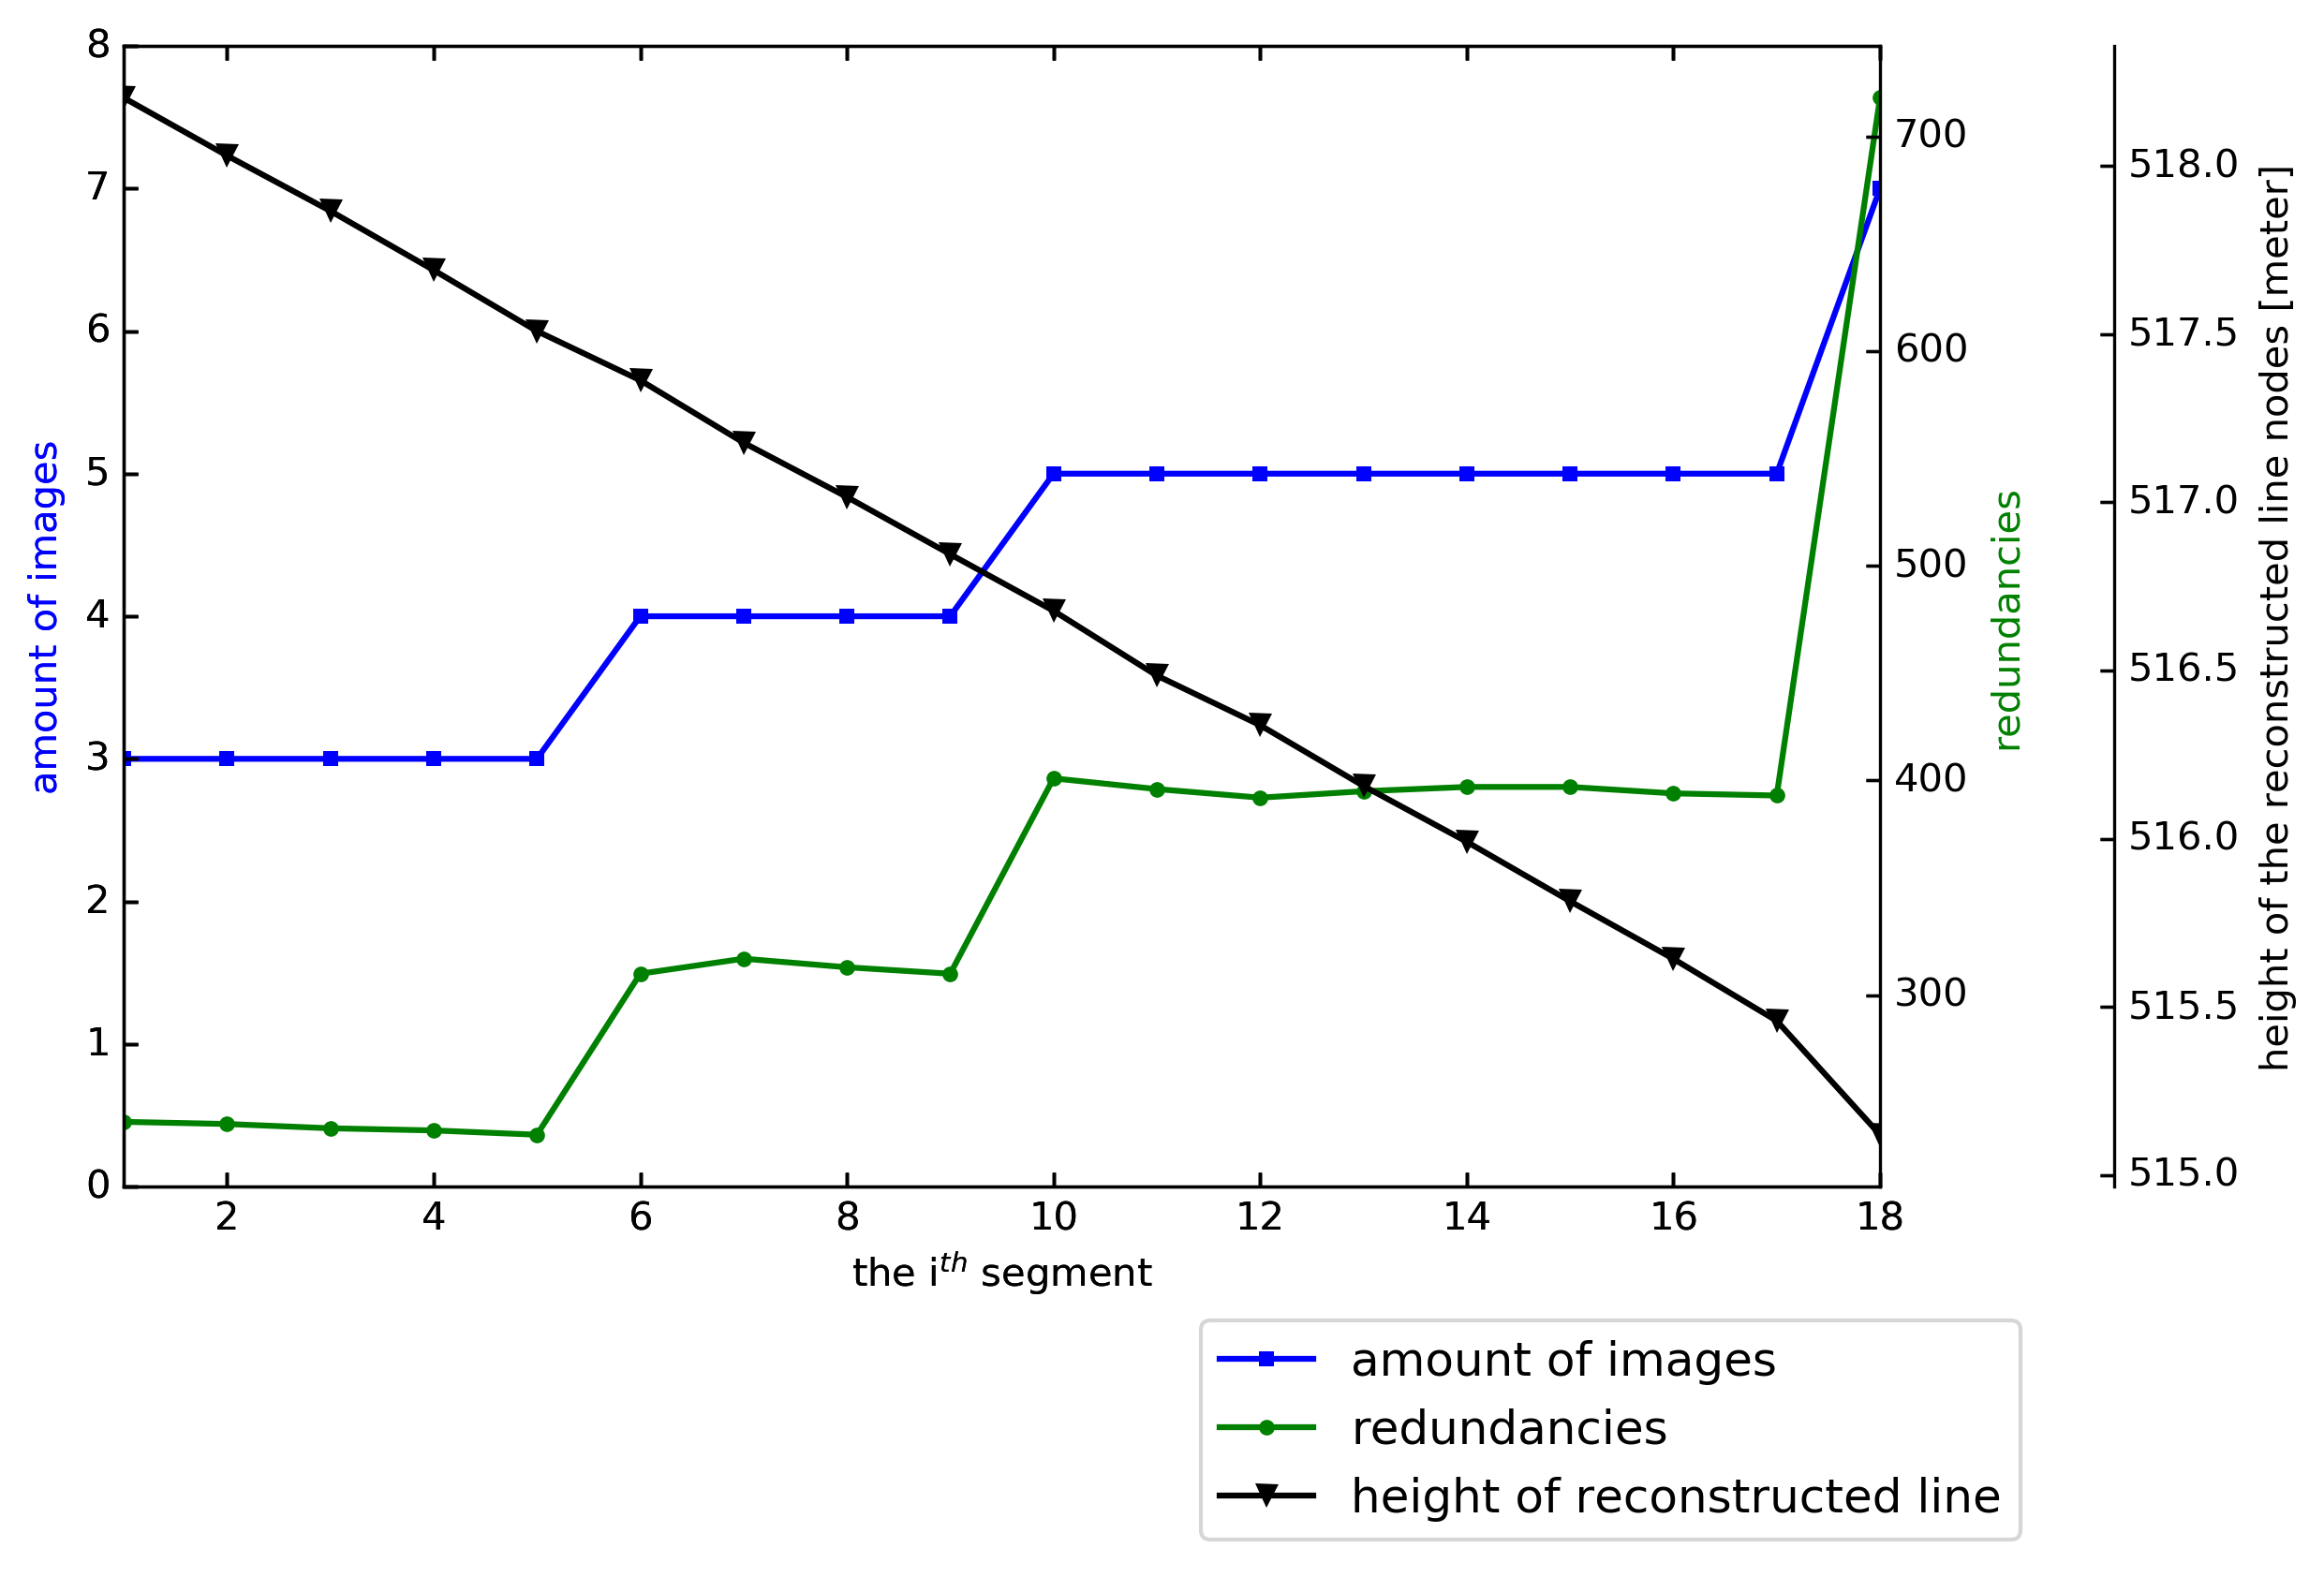
\includegraphics[width=\textwidth]{Simu_ImgNum.png}
  \caption{\small The amount of covering images, the redundancies and the height value of the reconstructed nodes, of each segment in simulation case.}
  \label{fig:SimuImgNum}
\end{figure}

%%% analysis on measurements:
\cref{fig:SimuError} shows the mean and variance of the added random Gaussian noise and the adjusted residuals of each segment. This two samples are compared by applying a two-tailed two-sample T-test. Null hypothesis and alternative hypothesis ($H_A$) are stated as:
\begin{equation*}
\begin{split}
H_0: \mu_1-\mu_2=0\\
H_A: \mu1-\mu_2\neq0
\end{split}
\end{equation*}

With significance level $\alpha=0.05$ and degree of freedom $\approx300$, the t-score is 
\begin{equation*}
T_{0.975,300}=1.968
\end{equation*}

As shown in \cref{fig:SimuTtest}, all the test statistics $T_{obs}$ of each segment are not less than $-T_{0.975,300}=-1.968$ or greater than $T_{0.975,300}=1.968$, i.e. not in the rejection region, the null hypothesis could not be rejected. In other words, we fail to claim that the adjusted residuals are statistically different from the added random noise.

%without the influence of imperfect camera parameters, 

\begin{figure}
  \centering
  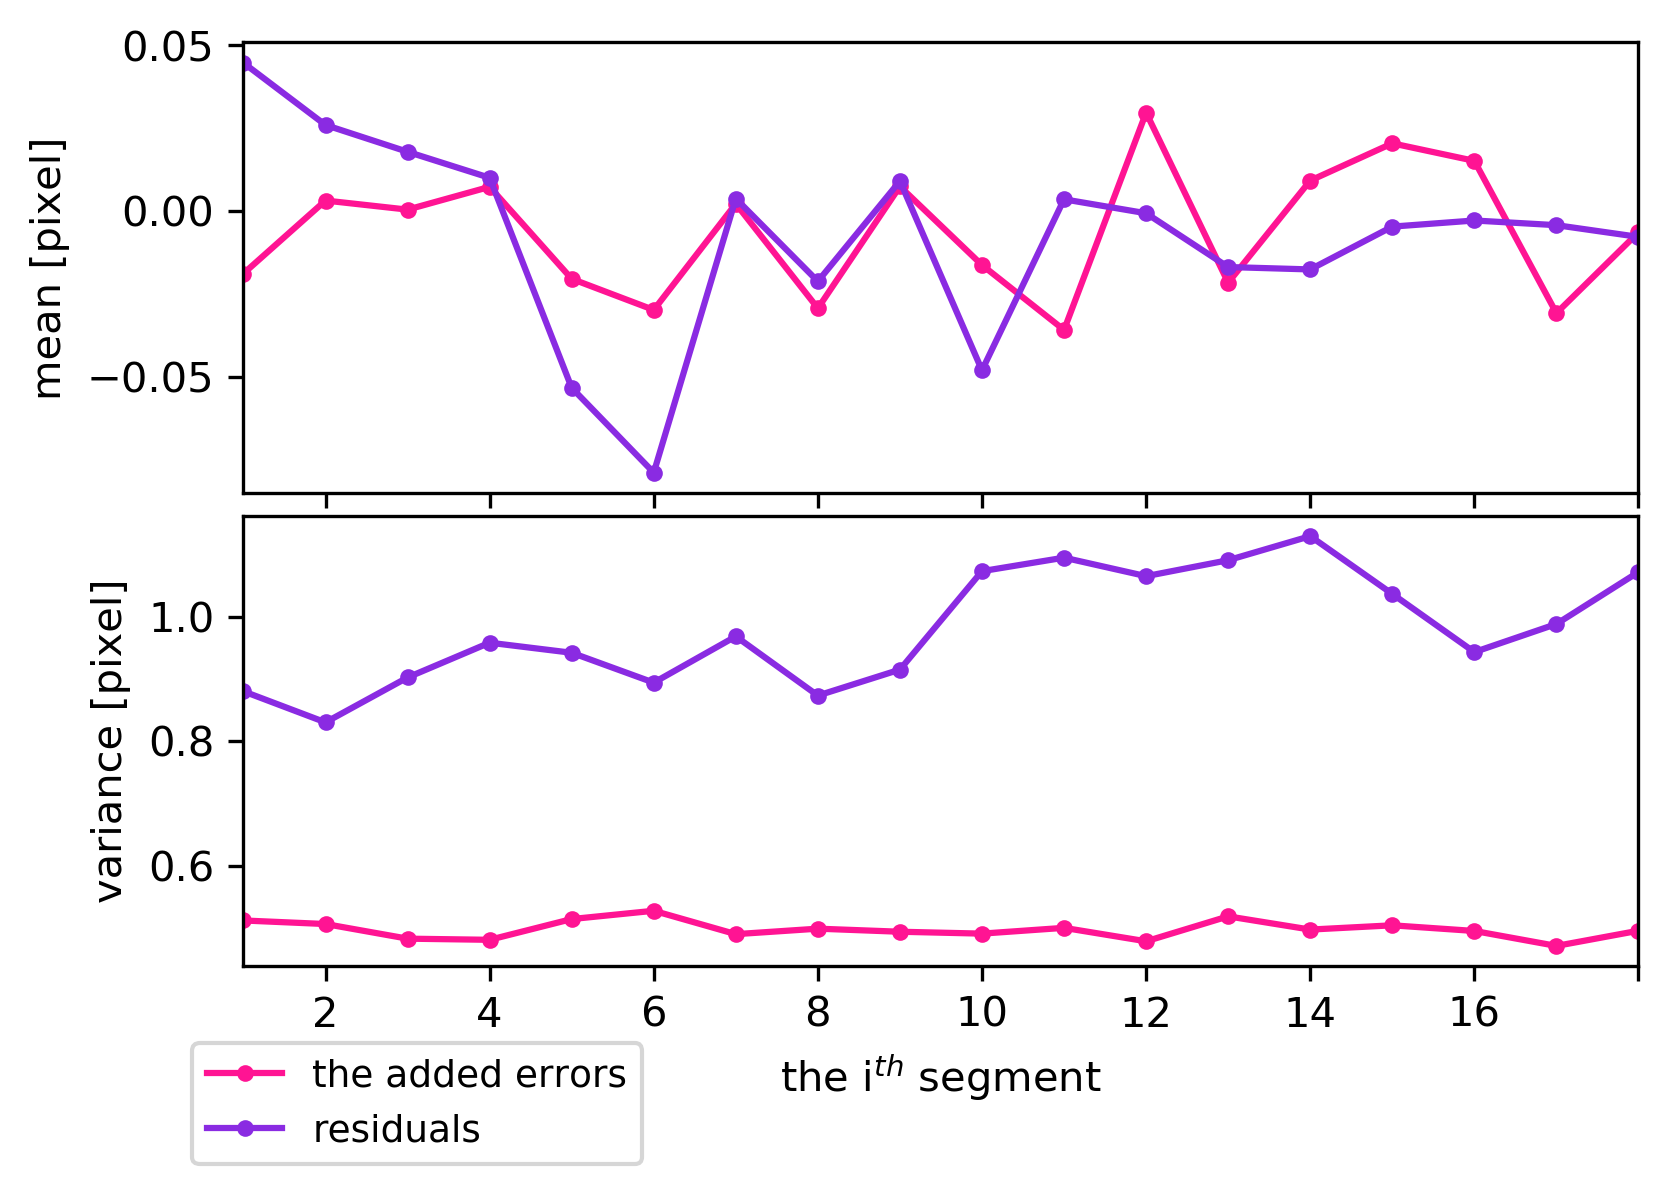
\includegraphics[width=0.95\textwidth]{Simu_error_1.png}
  \caption{\small The relation between the added random Gaussian noise and the adjusted residuals.}
  \label{fig:SimuError}
  \vspace{1cm}
  \centering
  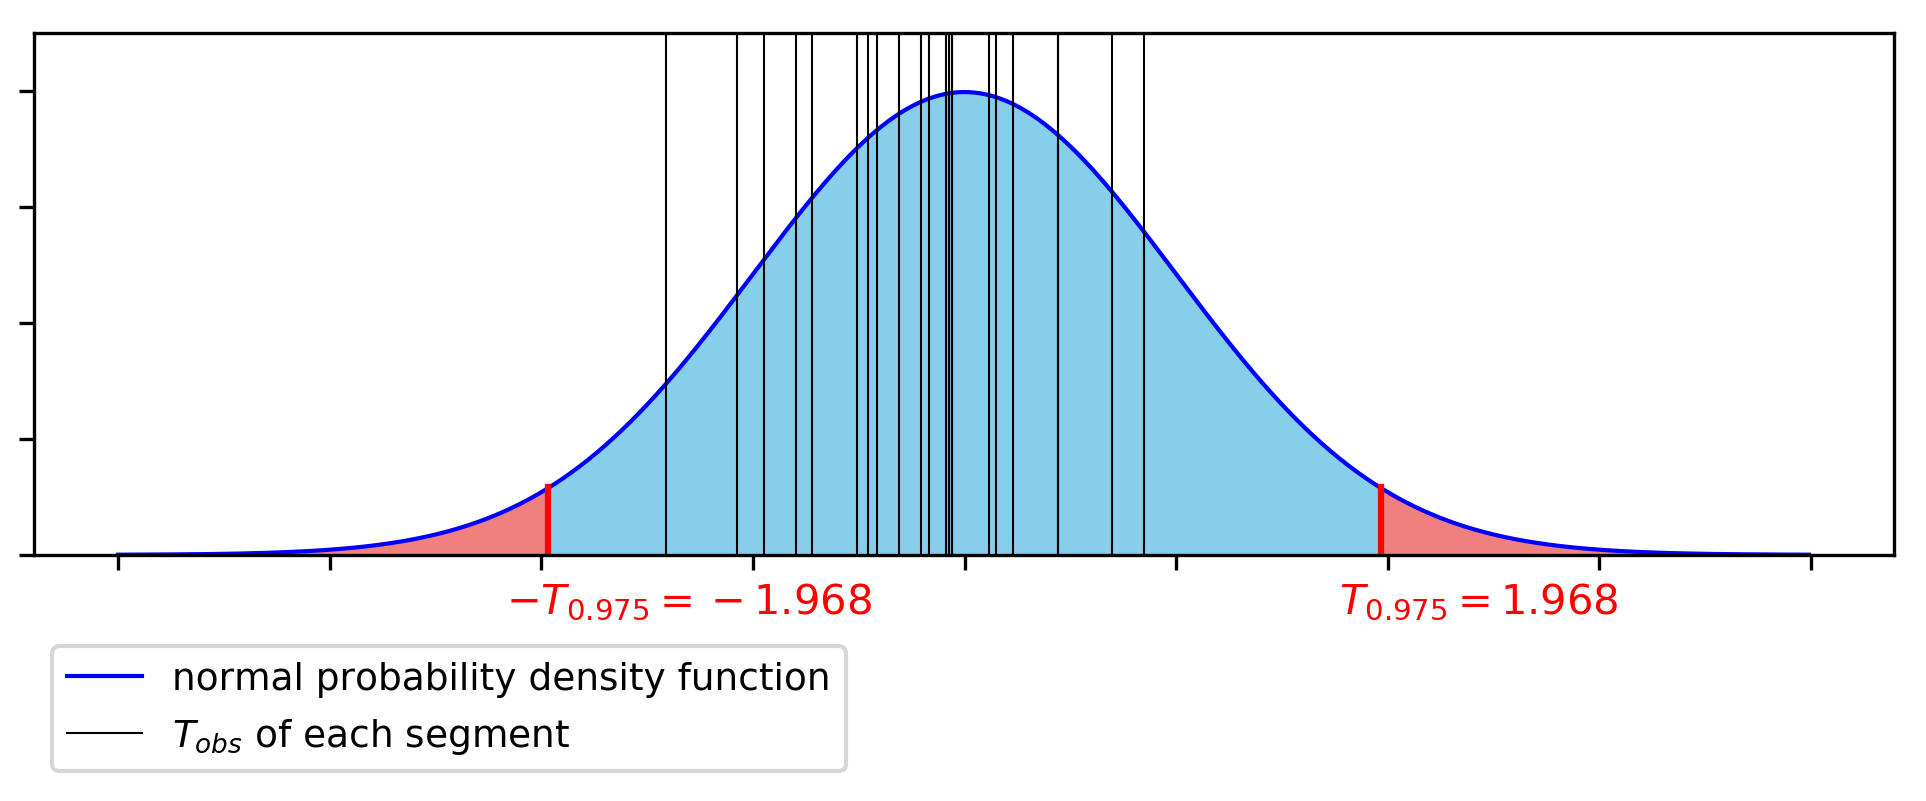
\includegraphics[width=\textwidth]{Simu_Ttest.png}
  \caption{\small The red area under the probability density function is the rejection region, which is 5\%. Since non of the $T_{obs}$ falls in the rejection region, the null hypothesis could not be rejected.}
  \label{fig:SimuTtest}
\end{figure}

\clearpage


By assuming a constant priori standard deviation of measurements to $1$ [pixel] in all the LS adjustment processes, the priori variance-covariance matrix of the estimated parameters
\begin{equation}
\Sigma_{\hat{X}\hat{X}}=\sigma_0^2(\mathsf{A^TA})^{-1}=
\begin{bmatrix}
\sigma_{\hat{X}}^2 && \sigma_{\hat{X}\hat{Y}} && \sigma_{\hat{X}\hat{Z}} \\
\sigma_{\hat{Y}\hat{X}} && \sigma_{\hat{Y}}^2 && \sigma_{\hat{Y}\hat{Z}} \\
\sigma_{\hat{Z}\hat{X}} && \sigma_{\hat{Z}\hat{Y}} && \sigma_{\hat{Z}}^2
\end{bmatrix}
\end{equation}
reflects the quality of the design matrix in different LS adjustment processes. In other words, by assuming same measuring quality of 1 pixel level in each segment, $\Sigma_{\hat{X}\hat{X}}$ reflects the configuration strength of each line segments.


From \cref{fig:SimuSigmaxx} it can be seen that the estimated parameters generally have smaller priori variance values (in horizontal direction) $\sqrt{\sigma_{\hat{X}}^2+\hat{\sigma}_{\hat{Y}}^2}$ and (in vertical direction) $\sigma_{\hat{Z}}$ with the increase of covering images. This tells that, {the precision of the estimated parameters can be improved by increasing the configuration strength, i.e. increasing the amount of covering images with different orientations}.

Besides, the priori variance of the estimated parameters is smaller in horizontal direction $\sqrt{\sigma_{\hat{X}}^2+\hat{\sigma}_{\hat{Y}}^2}$ than in vertical direction $\sigma_{\hat{Z}}$. This tells that {the reconstructed nodes have higher precision in horizontal direction}. 


\begin{figure}
  \centering
  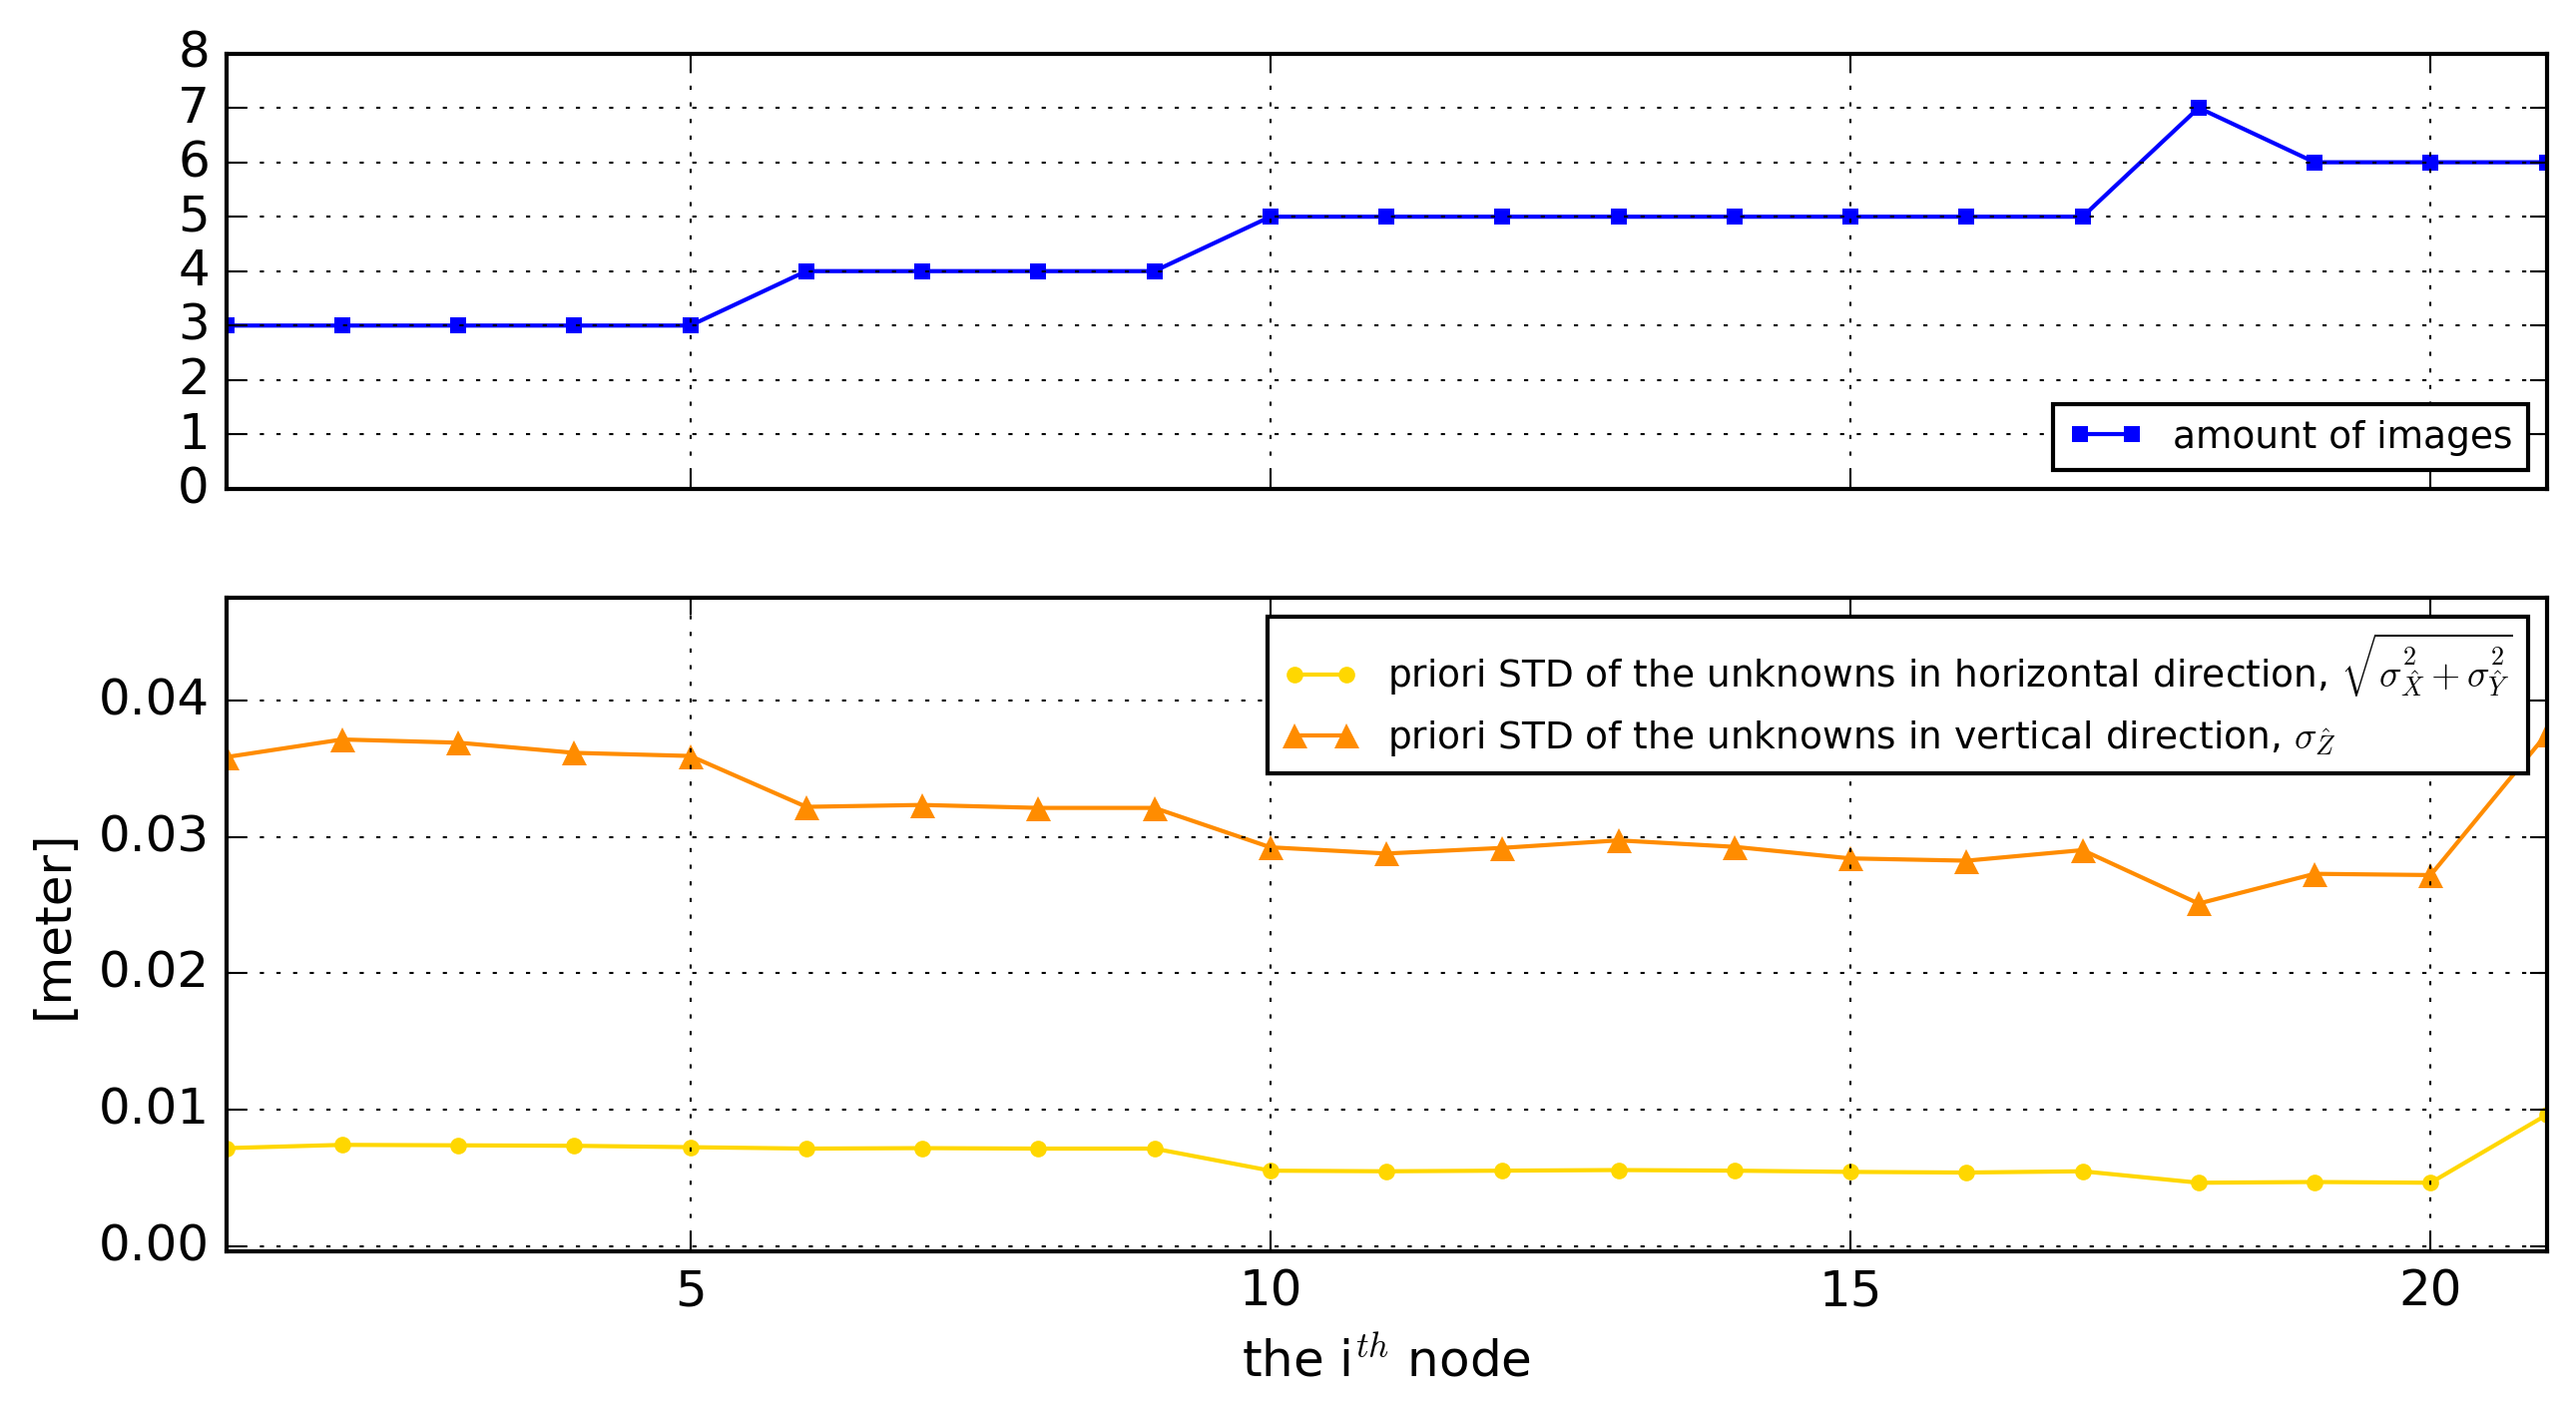
\includegraphics[width=\textwidth]{Simu_SigmaXX.png}
  \caption{\small The relation between the variances of the estimated parameters and the amount of images.}
  \label{fig:SimuSigmaxx}
\end{figure}

\clearpage
%%%%%%%%%%%%%%%%%%%%%%%%%%%%%%%%%%%%%%%%%%%%%%%%%%%%%%%%
\section{True Data}
\label{sec:truedata}

\subsection{True Data Result}
\label{subsec:trueresult}

A continuous lane marking of 255.9 meters length is reconstructed. \cref{fig:Test3D} shows the reconstructed line segments and the DSM profile in UTM 32N coordinate system. The distances from the reconstructed line segment to the DSM profile are computed and plotted into histogram in \cref{fig:TestHist}. They are collected along the reconstructed line segments with 0.2 meter spacing (considering the DSM grid of 0.2 meter), resulting in sample size of $1256$. The sample mean is $-0.181$ [meter] and the sample standard deviation is $0.174$ [meter]. %This sampling procedure is assumed to be independent and random.%??? and normal distributed (Z test assumptions)

Assuming DSM height profile being significantly lower than the reconstructed line segments for more than $17$??? centimeters, a lower-tailed Z-test is adopted. Null hypothesis ($H_0$) and (one-tailed) alternative hypothesis ($H_A$) are stated as:
\begin{equation*}
\begin{split}
H_0: \mu\geq-0.170\\
H_A: \mu<-0.170
\end{split}
\end{equation*}

A significance level $\alpha=0.05$ is selected, i.e. the area in body is $0.950$ out of 100\%. The corresponding z-score is:
\begin{equation*}
Z_{0.950}=1.64
\end{equation*}
leads to the decision rule: if $Z_{obs}$ is less than $-1.64$, reject the null hypothesis.

With the sample mean $\overline{x}=-0.181$ [meter],
the proposed population mean $\mu_0=-0.170$ [meter],
the sample standard deviation $\sigma=0.174$ [meter],
and sample size $n=1256$, the test statistic for a One Sample Z Test has a calculated value:
\begin{equation*}
Z_{obs} = \frac{\overline{x}-\mu_0}{\sigma/\sqrt{n}}=\frac{-0.181-(-0.170)}{0.174/\sqrt{1256}}\approx-2.24
\end{equation*}

As the test statistic $Z_{obs}\approx-2.24$ is less than $-Z_{0.95}=-1.64$, i.e. in the rejection region, the null hypothesis is rejected. In other words, {with 95\% confidence we can claim that the DSM profile is in average, statistically and significantly lower than the reconstructed line segments for at least $17$ centimeters in this region}. %This phenomenon is as expected, as mentioned in sec:DSM??? 

\begin{figure}
  \centering
  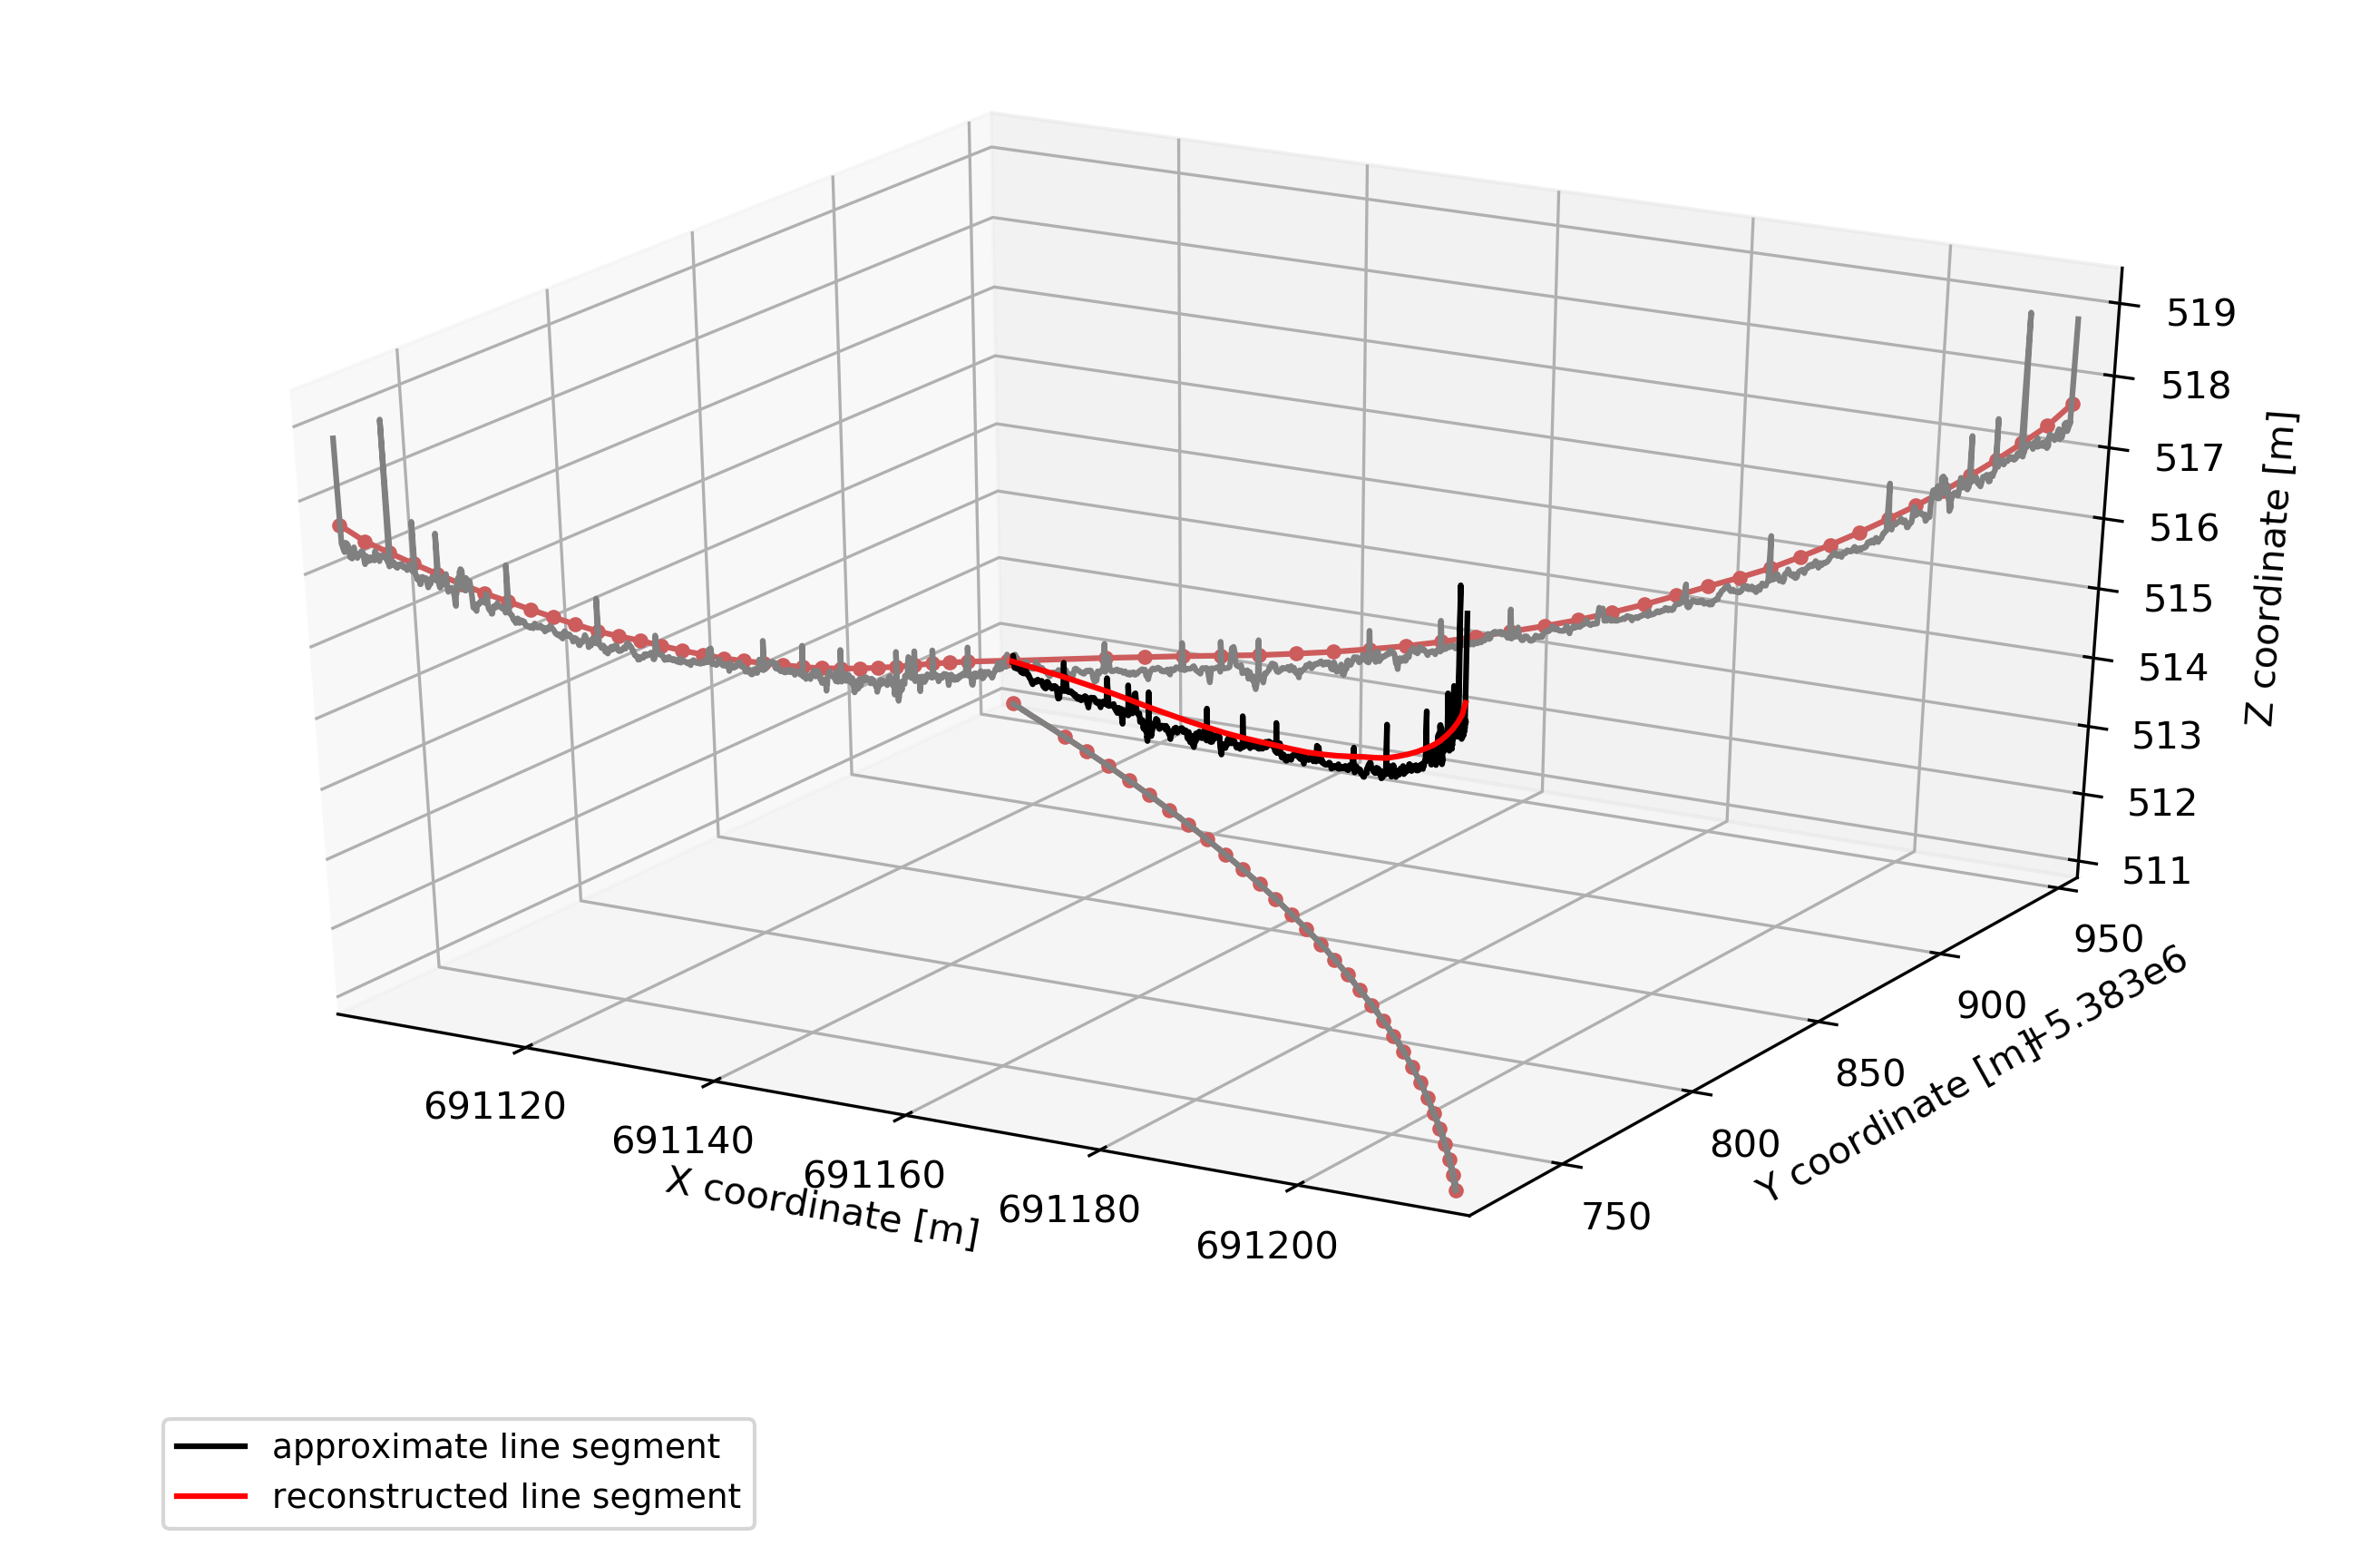
\includegraphics[width=\textwidth]{Test_3D.png}
  \caption{\small The reconstructed line segments and the unrefined DSM profile in UTM 32N coordinate system.}
  \label{fig:Test3D}
  \vspace{1cm}
  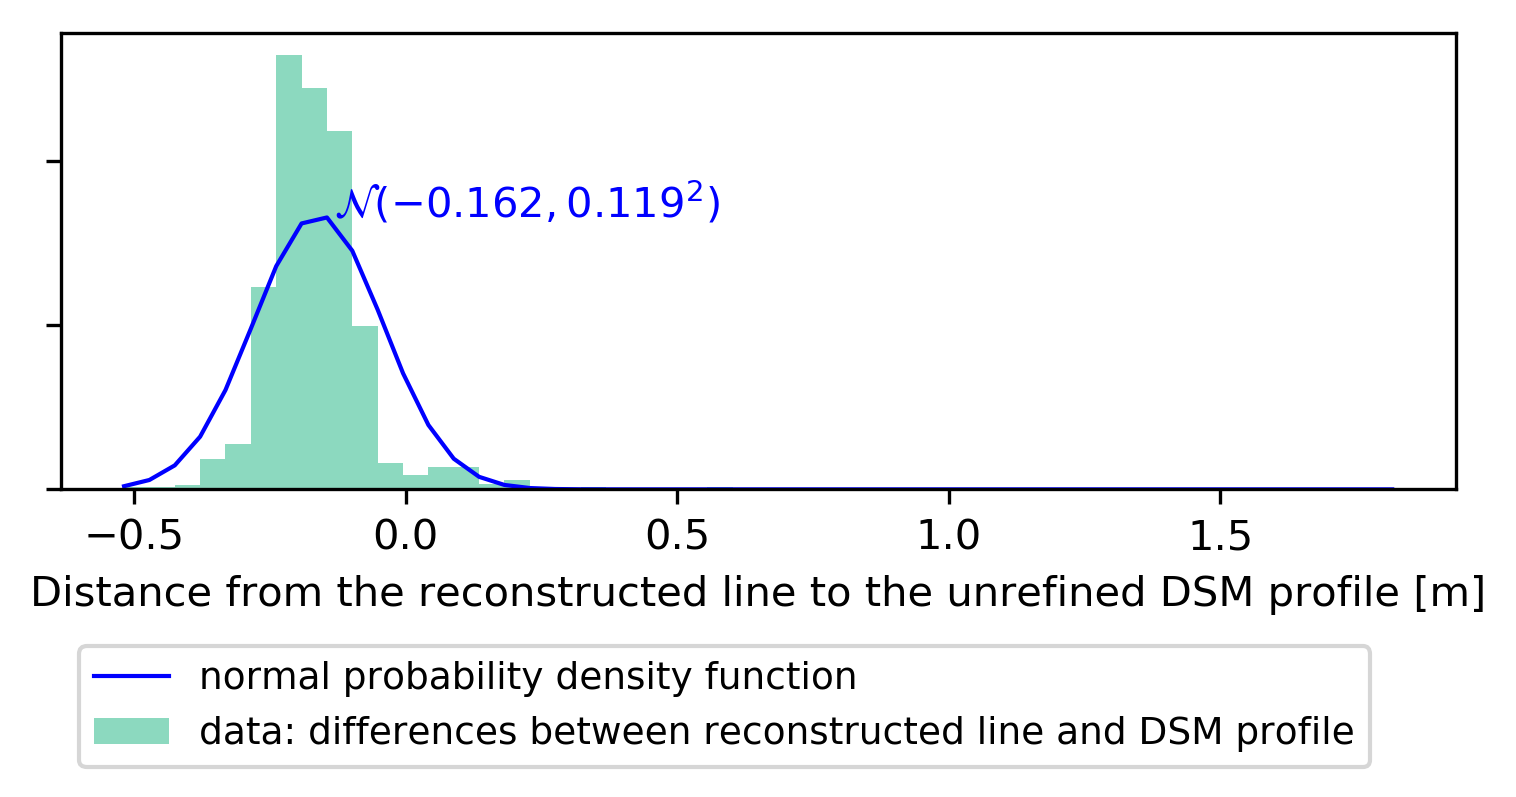
\includegraphics[width=\textwidth]{Test_hist.png}
  \caption{\small Histogram of the distances from the reconstructed line to the unrefined DSM profile.}
  \label{fig:TestHist}
\end{figure}

\clearpage

\cref{fig:TestImgNum} gives the information on the amount of covering images, the redundancies and the height value of the reconstructed nodes, of each segment. Note that in each segment, LS adjustment is processed independently.

\begin{figure}
  \centering
  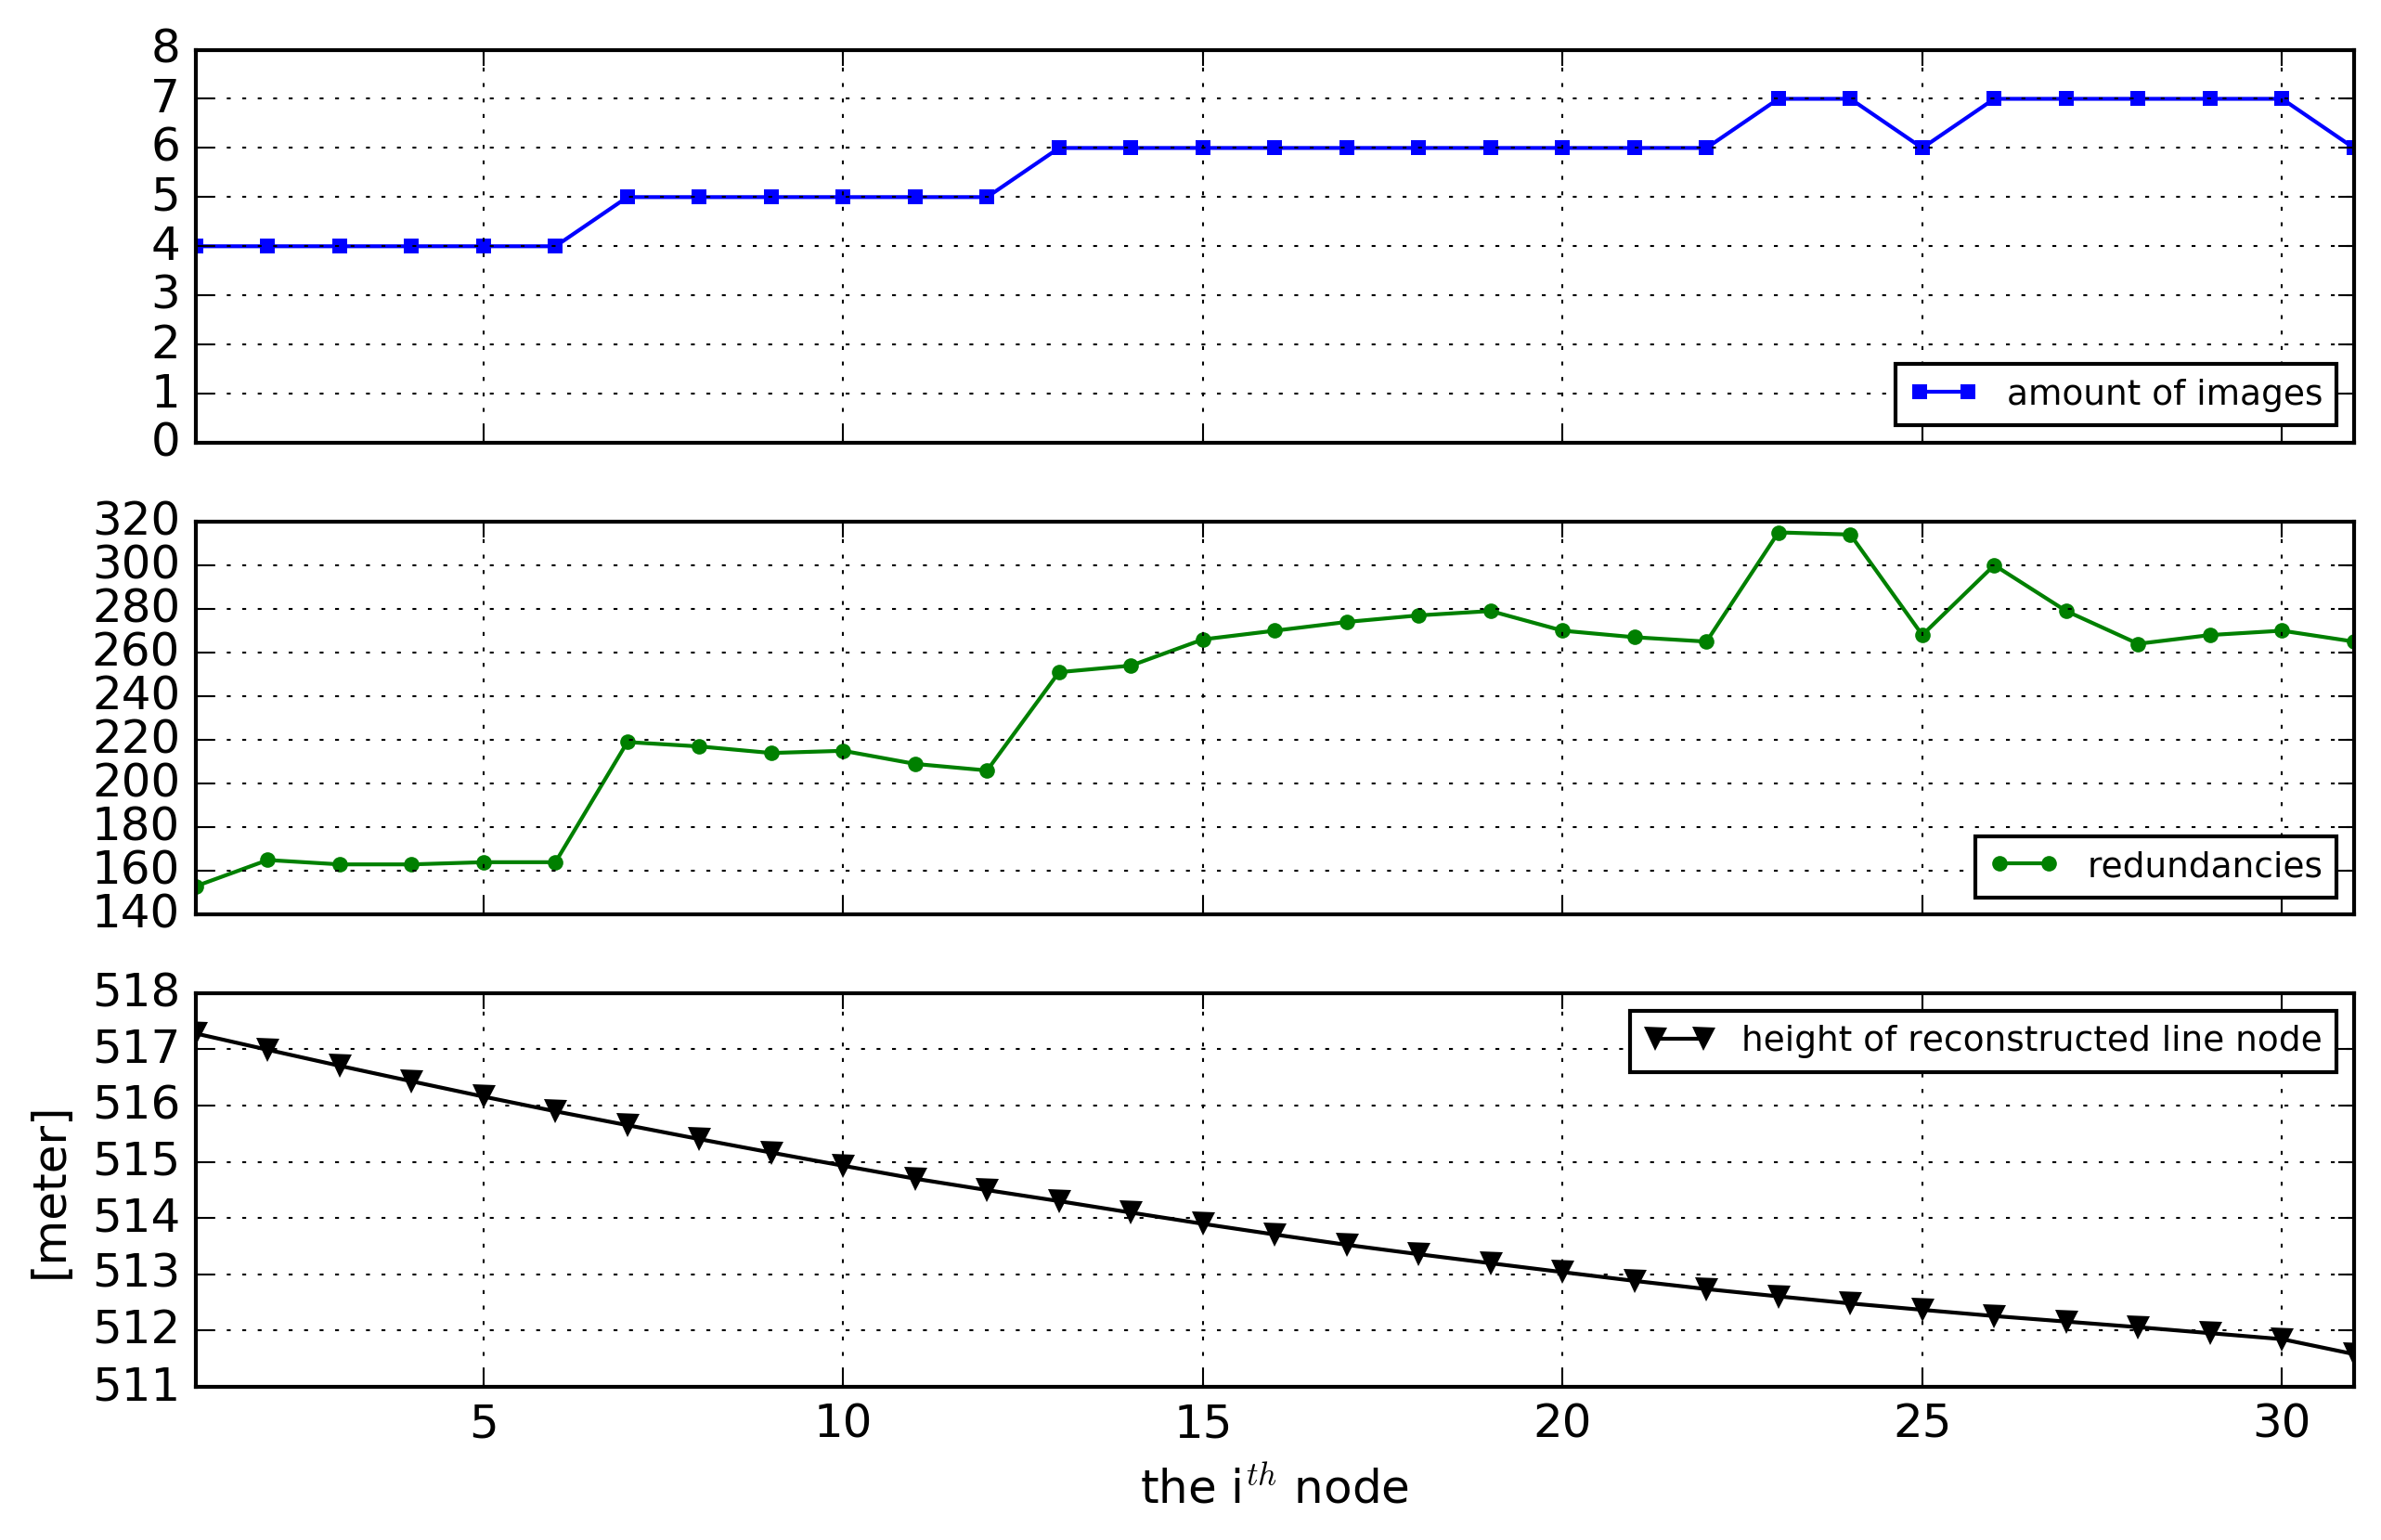
\includegraphics[width=0.95\textwidth]{Test_ImgNum.png}
  \caption{\small The amount of covering images, the redundancies and the height value of the reconstructed nodes, of each segment in the true data experiment.}
  \label{fig:TestImgNum}
\end{figure}


%\begin{figure}
%	\centering
%	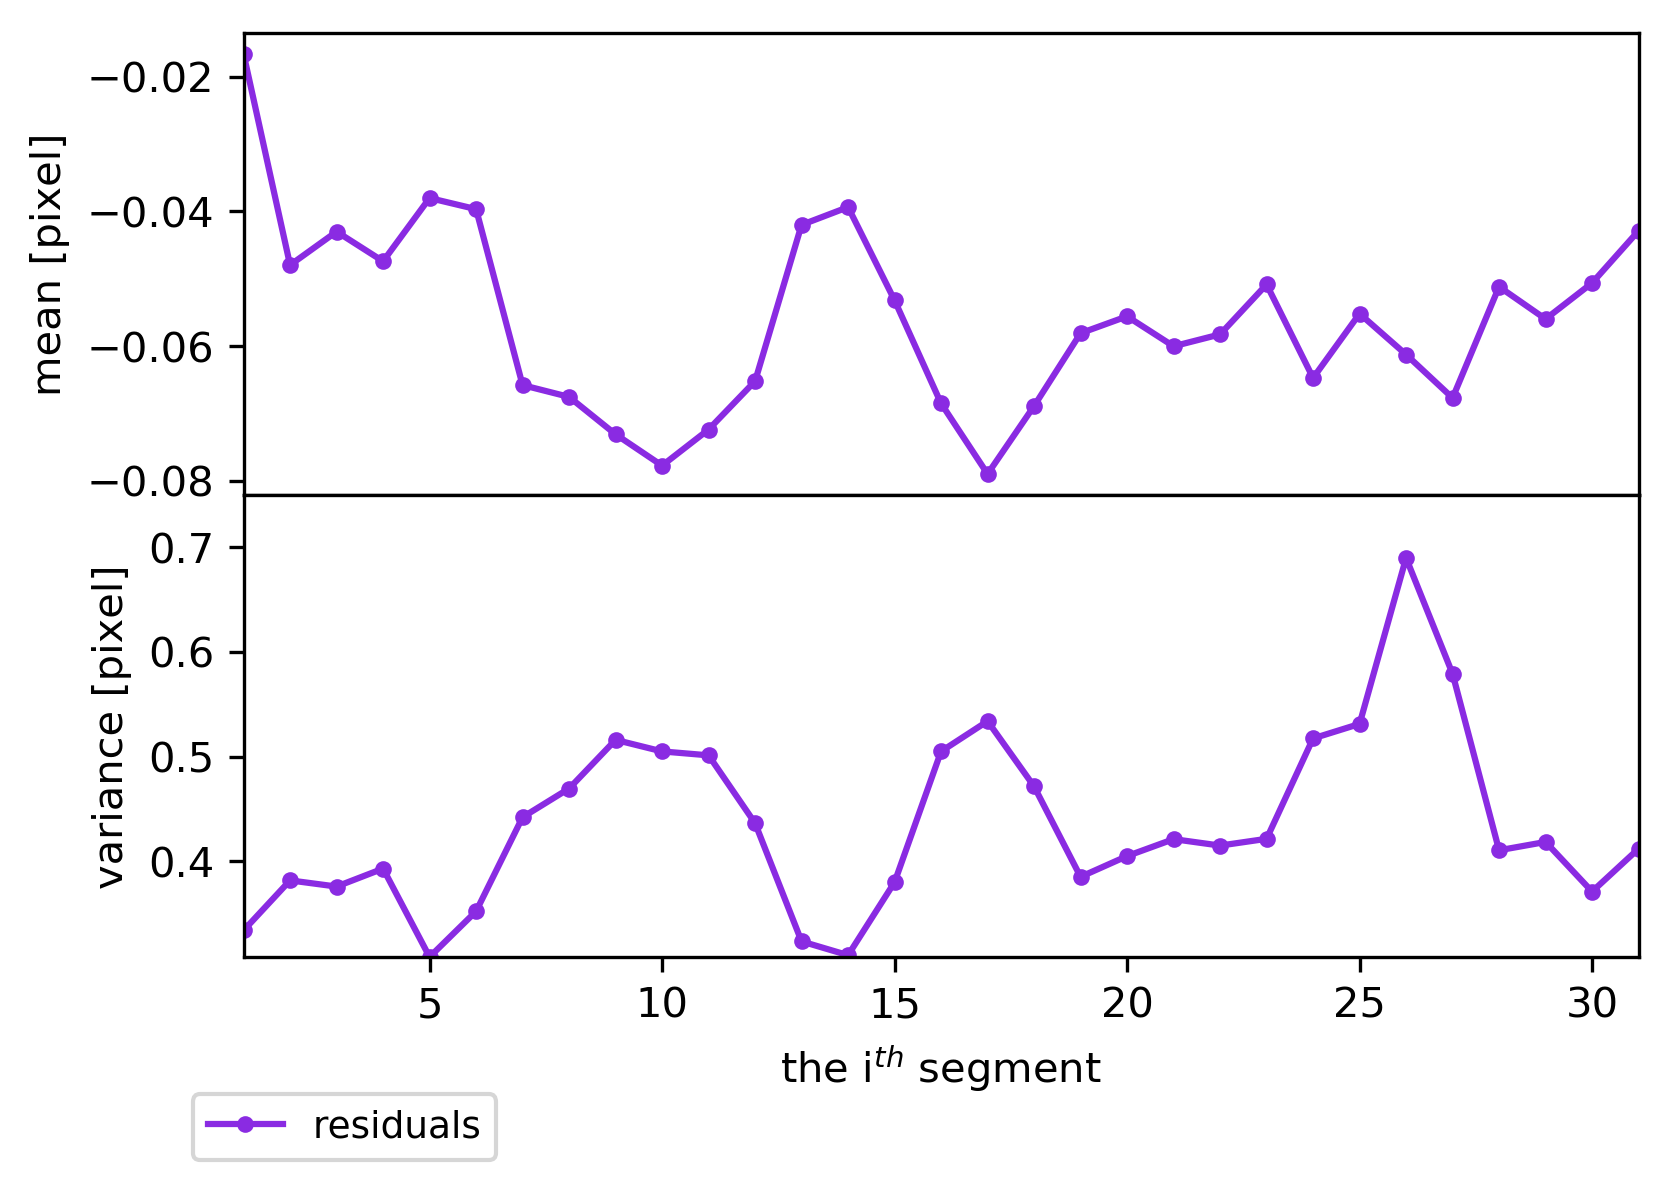
\includegraphics[width=0.8\textwidth]{Test_error.png}
%	\caption{\small Residual mean and posterior standard deviation.}
%	\label{fig:Testerror}
%\end{figure}


Compare to the simulation data, where all line segments lie on a straight line and have same orientations, the true data (a continuous lane marking) is a curve line, whose line segments have different orientations from each other. Even some segments may have same image coverage configuration, their LS model may have different configuration due to their different orientaions in 3D space. \cref{fig:TestSigmxx} shows that the estimated parameters generally have smaller priori variance values with the increase of covering images. However there are some other factors influencing the configuration strength with same covering image amount.(vermutlich, the configuration strength in image space counts. show figures)

By increasing the configuration strength, the priori precision of the estimated parameters can be improved. {Not only the increase of the amount of covering images but also the line segment orientations in image space count for the configuration strength}.

\begin{figure}
  \centering
  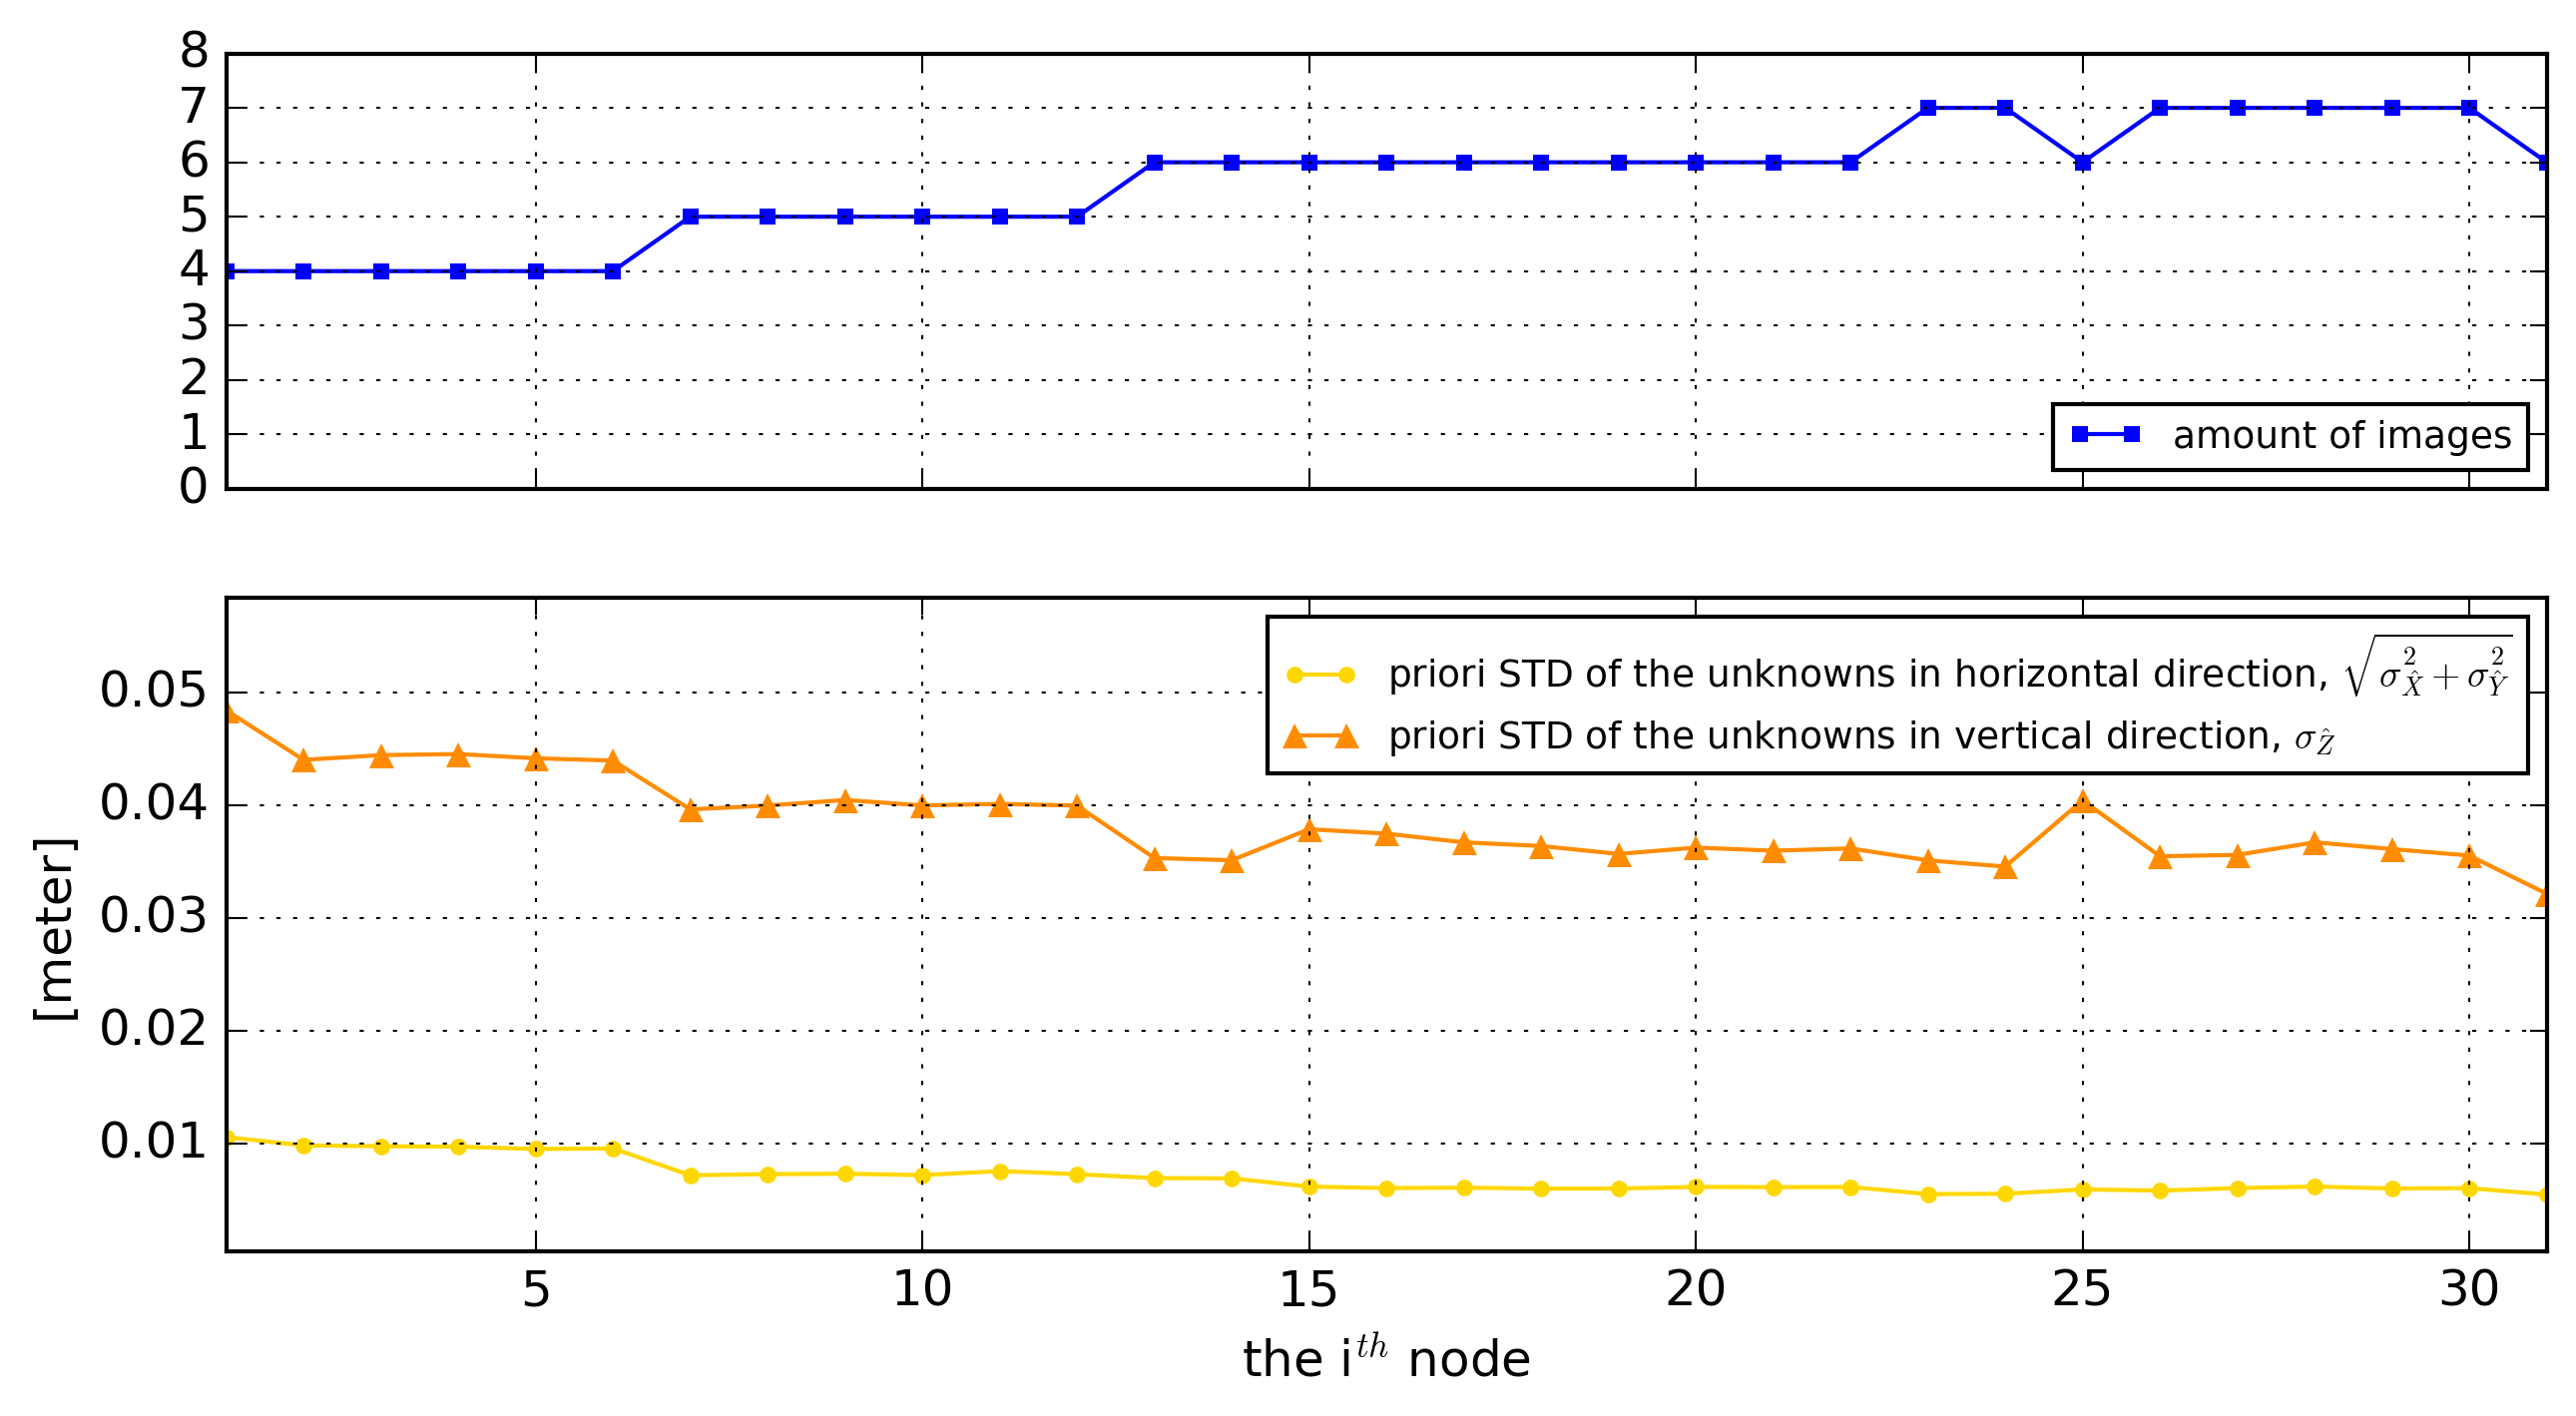
\includegraphics[width=\textwidth]{Test_SigmaXX.png}
  \caption{\small The variances of the estimated object coordinates, in horizontal and vertical directions.}
  \label{fig:TestSigmxx}
  \vspace{0.5cm}
  \centering
  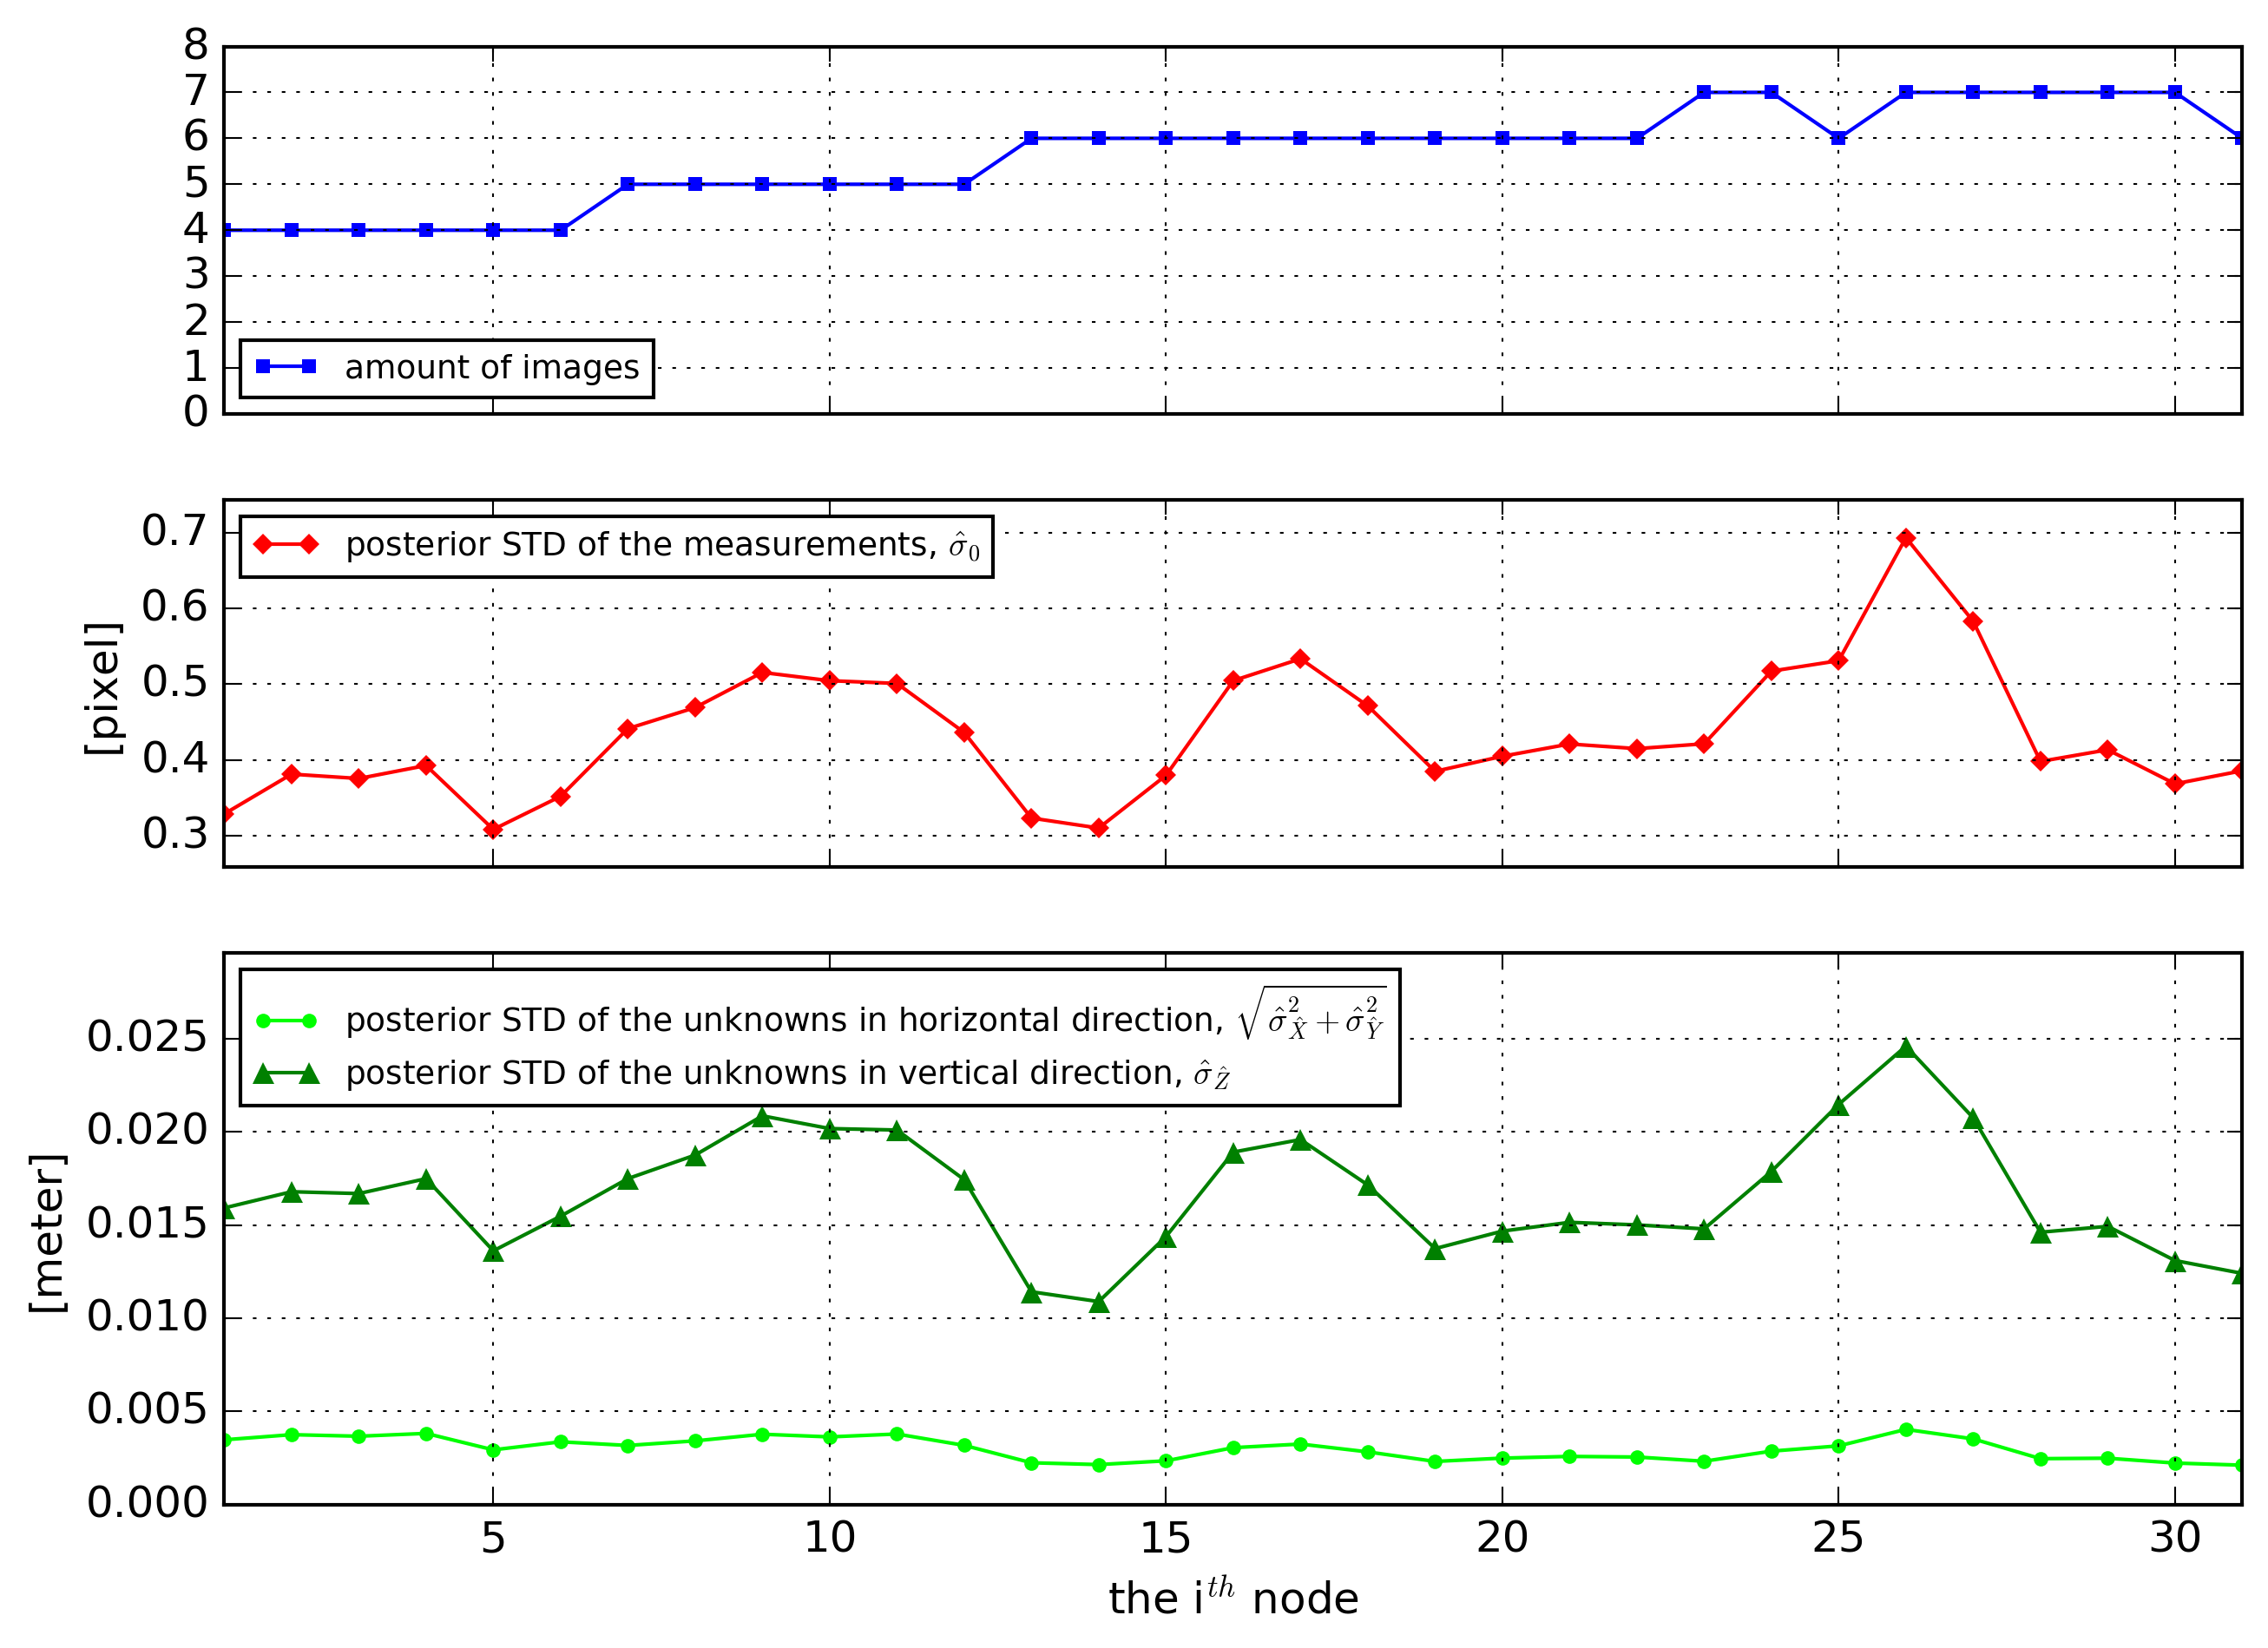
\includegraphics[width=\textwidth]{Test_SigmaXXhat.png}
  \caption{\small The estimated variances of the estimated object coordinates, in horizontal and vertical directions.}
  \label{fig:TestSigmxxhat}
\end{figure}

The reconstructed lane-markings in the testing area are shown in \cref{fig:TestAll3D} and \cref{fig:TestAll2D}. 

\begin{figure}
	\centering
	\subfloat[]{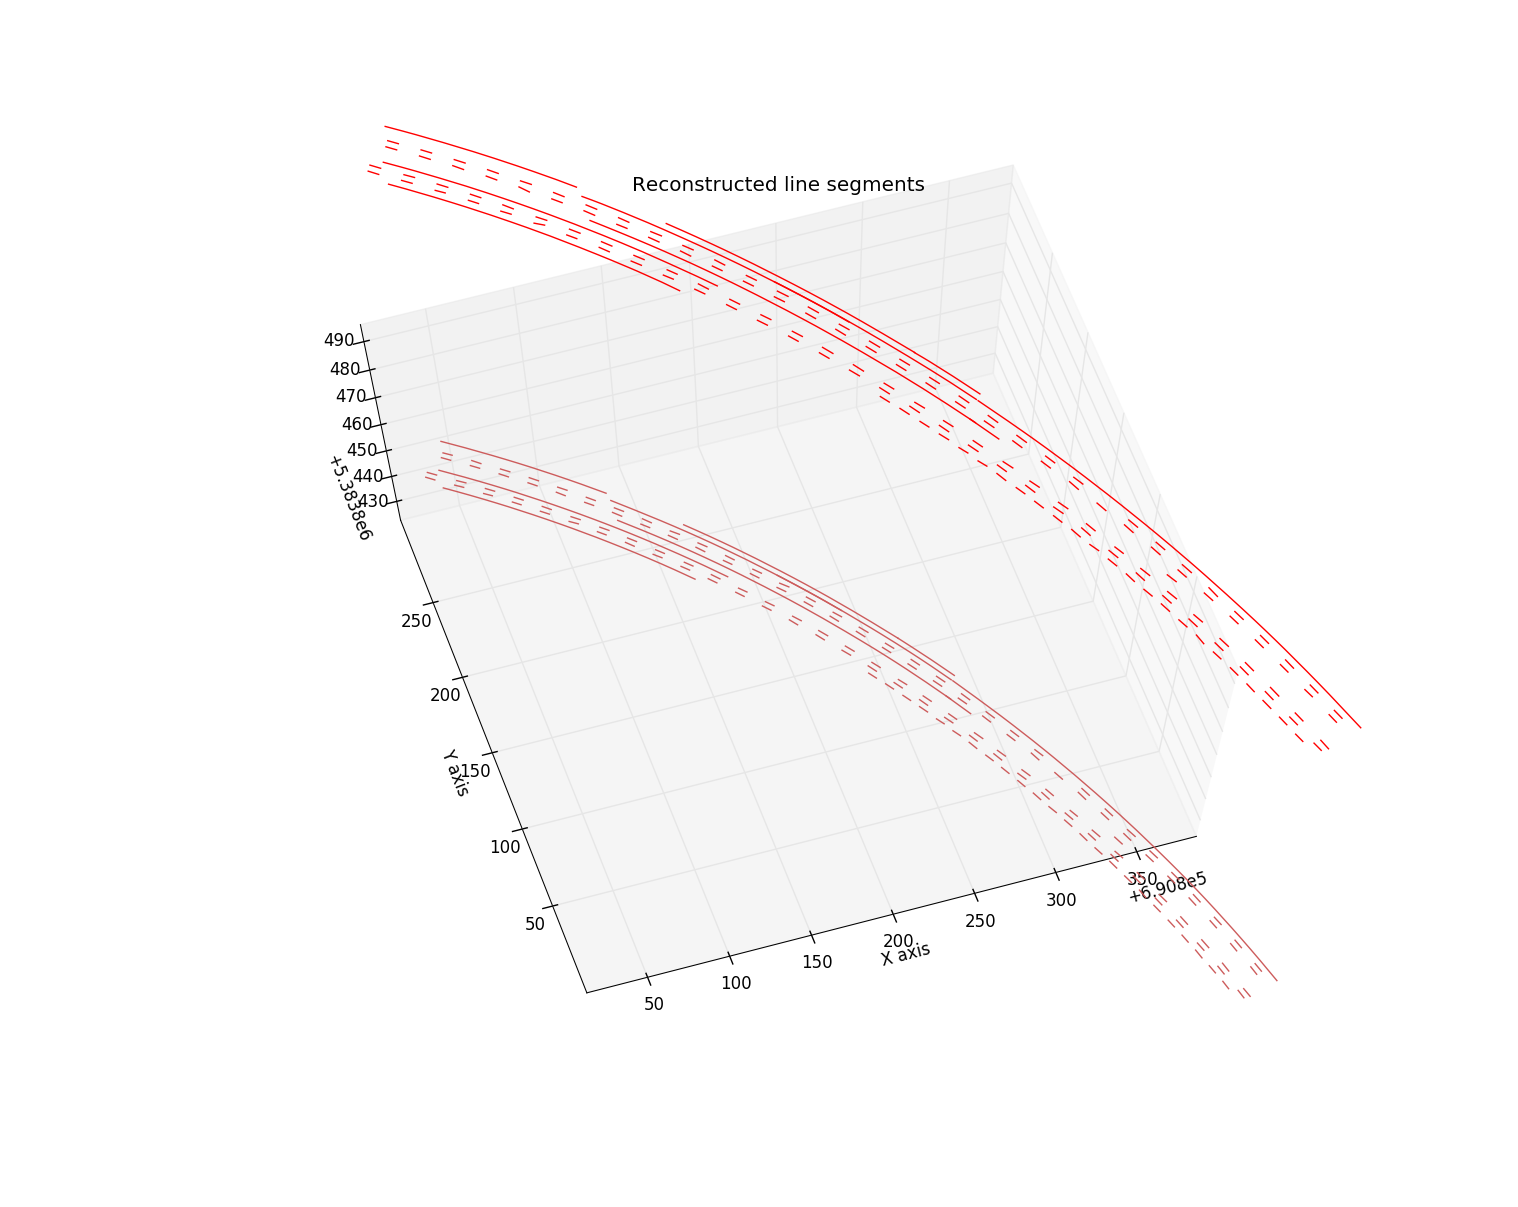
\includegraphics[width=0.8\textwidth]{Reconstructed_BeforeandAfter.png}}
	
	\subfloat[\small Zoom in to show the difference between the original DSM profiles and the reconstructed lines.]{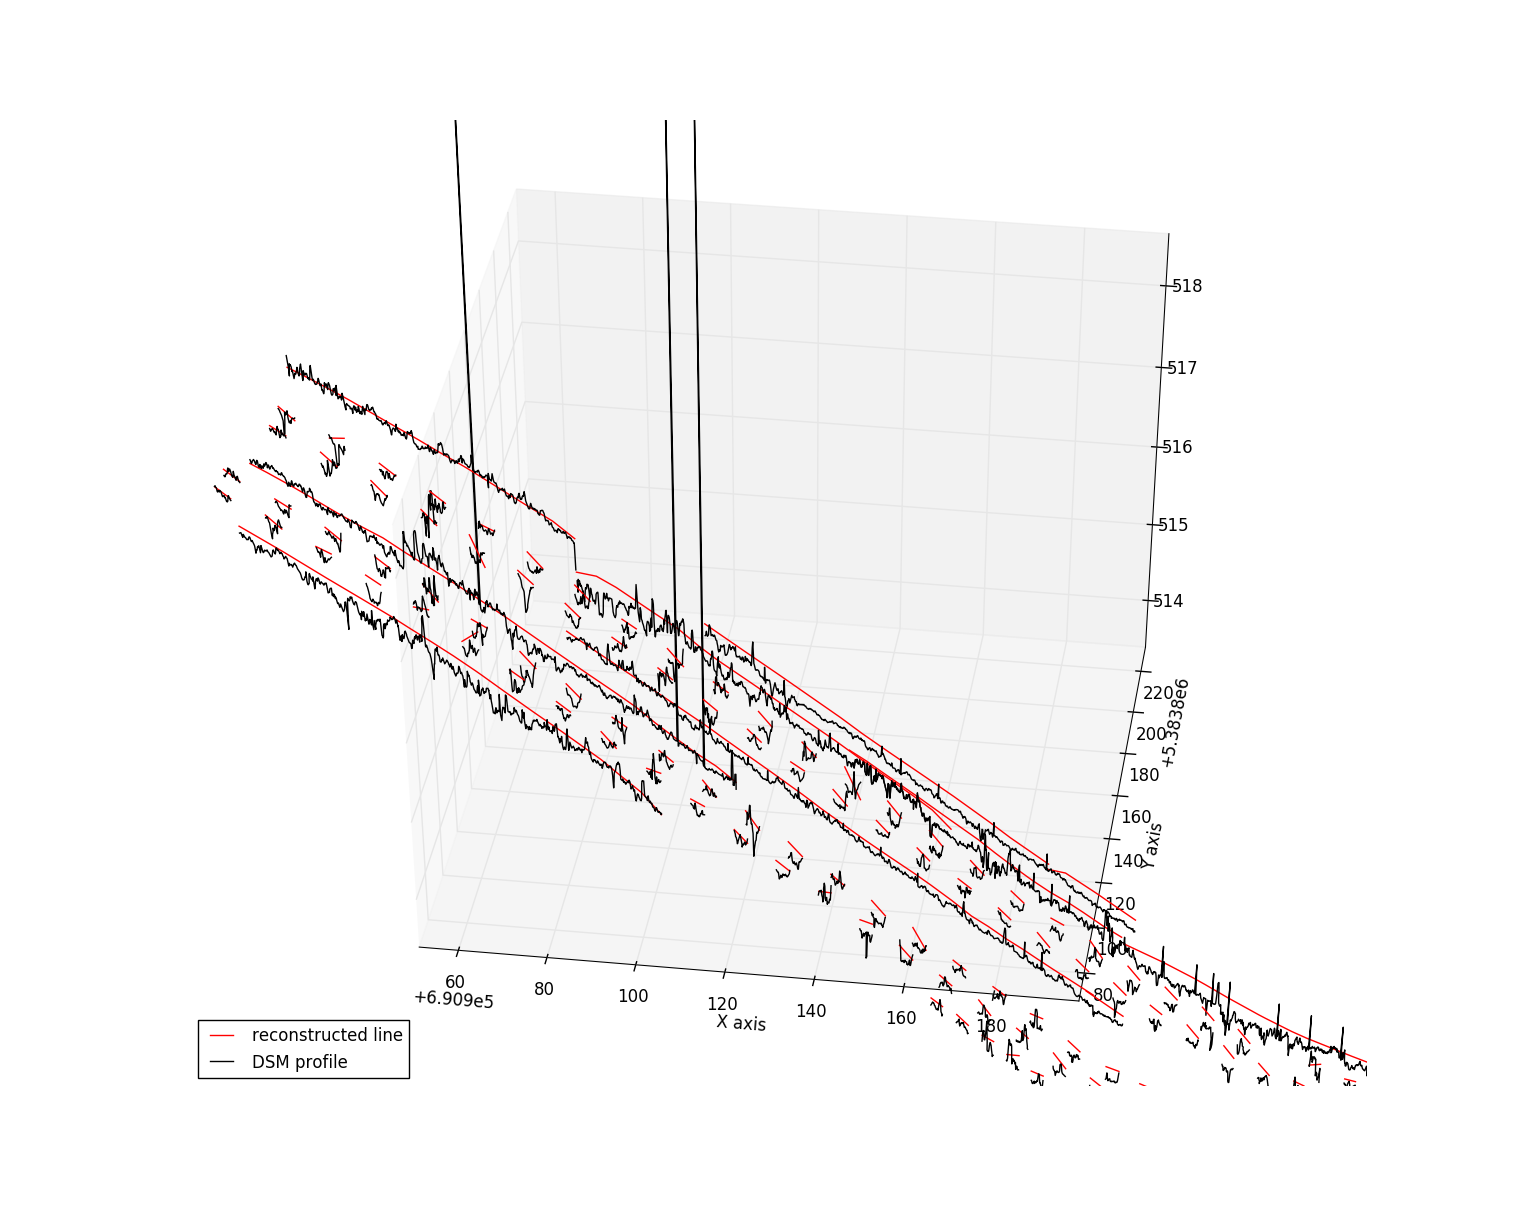
\includegraphics[width=0.8\textwidth]{Reconstruction_zoom3.png}}
	\caption{\small All the reconstructed lane-lines in the testing area.}
	\label{fig:TestAll3D}
\end{figure}

\begin{figure}
	\centering
	\subfloat[]{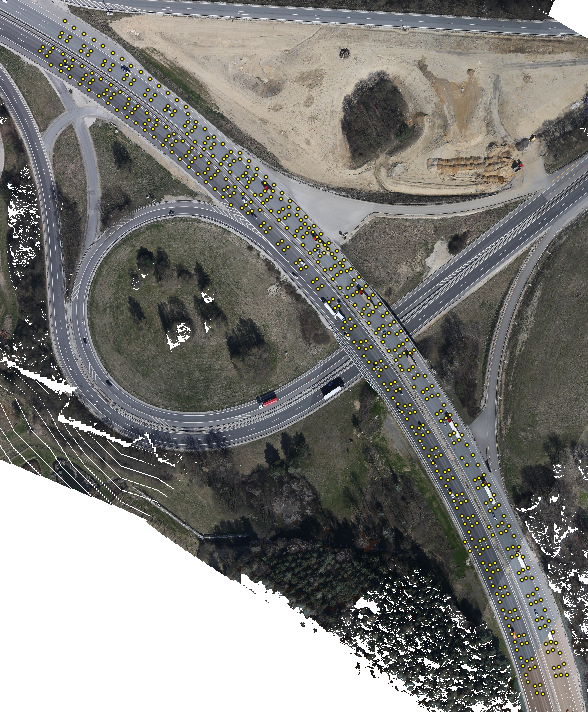
\includegraphics[width=0.9\textwidth, trim=0 12 0 17,clip]{all_1.png}}
	
	\subfloat[Zooming into road surface]{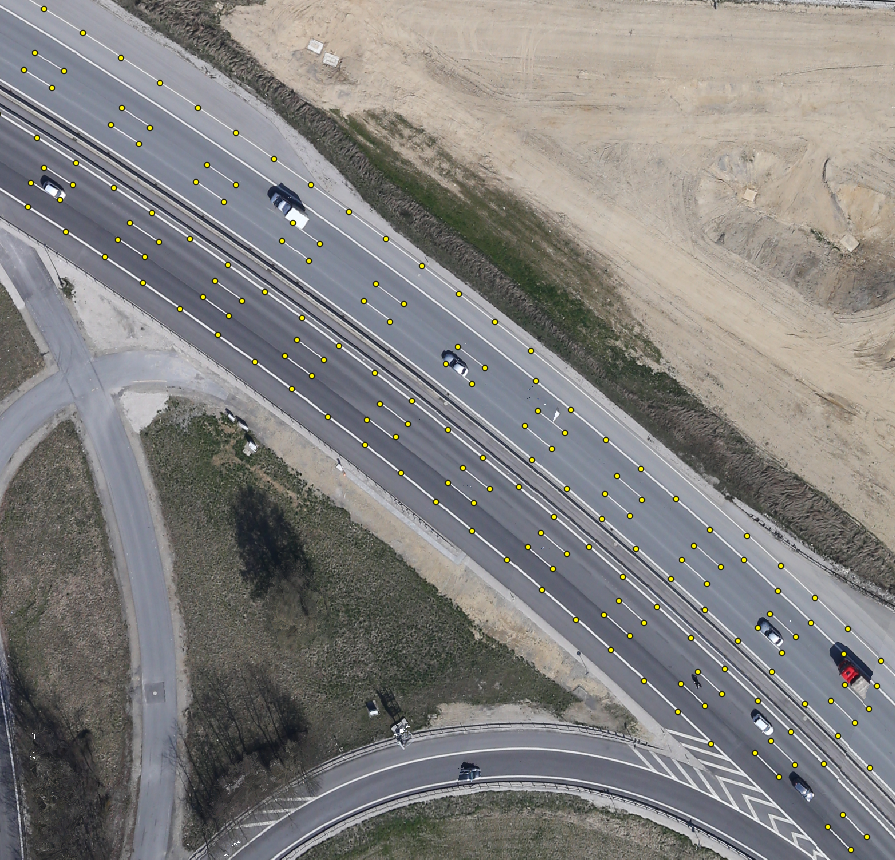
\includegraphics[width=0.9\textwidth, trim=150 350 130 300,clip]{all_2.png}}
	
	\caption{\small All the nodes of reconstructed lines on georeferenced aerial images, in UTM 32N coordiate system.}
	\label{fig:TestAll2D}
\end{figure}

